\documentclass[12pt,a4paper]{article}

\usepackage[T1]{fontenc}
\usepackage[latin1]{inputenc}
\usepackage{graphicx}
\usepackage{upquote}

\begin{document}
\title{%
    \begin{minipage}\linewidth
        \centering\bfseries\sffamily
        PID : Packaging - Integration - Development 
        \vskip3pt
        \large An integrated software development process
        	\vskip3pt
        	\large Tutorial Document
    \end{minipage}
}

\author{
	Robin Passama\\
	CNRS Research Engineer\\
	Robotic Department\\	
	LIRMM - UMR5506 - University Of Montpellier\\	
	\texttt{passama@lirmm.fr}}
\date{October 2013}

\maketitle

\bigskip
\bigskip
\bigskip
\bigskip
\bigskip
\bigskip

\begin{figure}
\center

\includegraphics[scale=0.7]{images/logos_officiels.png}
\end{figure}

\pagebreak

\section*{Introduction}
The main goal of this document is to provide a method that helps improving the overall quality of the code and applications produced by the robotics department of LIRMM. By improving the quality we aim at:
\begin{itemize}
\item simplifying the understanding and the modification of code produced by others.
\item simplifying the reuse of software components we develop.
\item pooling software developments between robotic teams.
\end{itemize}

To achieve this goal the Finding, Writing, Compiling, Testing, Version controlling and Documenting of the code are mandatory concerns. This document define how the whole development process is organized.

\section{Basic Concepts}

The following subsections explain basic concepts that need to be understood to start working with the PID methodology. First of all, root concepts are:

\begin{itemize}

\item \textbf{package} : a package is the basic unit for code development, unit testing, source version controlling, deployment specification, documentation writing. A package provides some functional code that can be reused (libraries, executables, header files, scripts, etc.) and depends on other packages either for its compilation (static libraries, header files archives/folders) or for its runtime use (dynamic libraries, executables, script-like files). It can contains as well an entire huge software (e.g. operating system) as a very elementary piece of code (e.g. header files, a library, etc.).A package has two main different forms :
\begin{itemize}
\item a source form. In this form, the package is a git repository that contains the  package's source code. It is something "alive" that is continuously evolving along development process.
\item a binary form. In this form, the package is a collection of software artefacts (headers, configuration files, executables, libraries, documentation, etc.) deployed in a given place of a file system. It is something static (does not evolved) that is associated to a specific version of the package's source form. A binary package can be embedded into an archive in order to be easily retrieved and deployed on a file system.
\end{itemize}

\item \textbf{workspace}:  the workspace is the folder hierarchy in which the user develops source packages and deploys the binary packages he uses (third party or resulting from its own package deployment). The basic idea is to avoid to use system dependencies : every software artefact in the development process is then local and relative to the workspace, except of course artefacts bound to system dependencies. 

\item \textbf{package server} : a package server is a computer (accessible across the network) that hosts many packages (either source or binary). It centralizes the access to packages, and handles the rights of the users for each package. It is responsible of the global version control of packages. It can also provides tools to manage the development of packages it hosts (teams members, bugs and activities tracking/reports, wiki, version history and development branches, visualization, etc.).
\end{itemize}
 
The present document helps normalizing the development of packages inside workspace, and the way packages and workspaces are managed on development servers. As definition of concept and process is intrinsically bound to the concepts and process involved in the software tools used, the section first quickly present these tools. Then we define core concepts of the PID methodology based on those of the tools.
 
\subsection{Tooling}

For each development task in a package, a tool is used to achieve this task. To ease the portability of code, only \textbf{cross platforms} tools are used:
\begin{itemize}
\item \textbf{git} is used for the concurrent version control and patching of the code. It is also the tool used to deliver and retrieve the source code.
\item \textbf{cmake} is used to manage the build process, but also deployment and test.
\item \textbf{doxygen} is used to generate api documentation of source code.
\item \textbf{latex} is the preferred language to write documents, since it allows to version the full content of file (raw text and structure of the document), as opposed to binary formats like Microsoft Word or Libre-Office that are not well handled by git.
\end{itemize}

Other tools used, like the compiler/linker (e.g. gcc) used with cmake, or the ssh agent used with git, or even development environment (e.g. Xcode, Eclipse) interfaced with cmake, git and doxygen, are supposed to be native (i.e. specific to the OS used) and so adapted by the user depending on the platform he uses and his own preferences.

\subsection{Package}

The package is the basic working unit for developers. A package :
\begin{itemize}
\item contains the functional source code.
\item contains the tests source code.
\item contains version control information files.
\item contains the compilation files used to : build the source code and documentation, run tests, generate configuration files, install its resulting binary form in the workspace and generate an installable archive of its binary form.
\end{itemize}

The main idea is that a package is self-explanatory. It does not means it contains all code and artefacts it requires but it contains all information needed to satisfy its dependencies. In other words considering a given package, its installation process is done using this information and the information contained in its dependent packages.

\subsubsection{Package Structure}

A Package is generically structured according to the folder hierarchy defined below:
\begin{itemize}
\item the root folder of the package has the \textbf{name of the package}. This folder is basically a git repository which allows to manage concurrent work and version control on a package's content.
\item the \textbf{.git} folder contains version control related information, automatically managed by the git tool.
\item the root \textbf{.gitignore} file is used to exclude from version control some artefacts like temporary files.
\item the \textbf{CMakeList.txt} file is used to describe how to build, install and test the whole package. It also contains meta-information on the package (authors and institutions, repository address, license, etc.).
\item the \textbf{build} folder contains results from build process and contains two subdirectories: \textbf{release} and \textbf{debug}. Each of them contains the hierarchy of files and artefacts generated by the compilation process.
\item the \textbf{src} folder contains sources files (.c/.cpp/.cc in C/C++) of libraries. Each subdirectory of \textbf{src} contains sources use to build one or more library and is itself hierarchically organized according to developers needs. Libraries provided by the package are defined by the CMakeList.txt file contained in the \textbf{src} folder.
\item the \textbf{include} folder contains interface description files, typically exported (i.e. installed) headers files (.h, .hpp, .hh) in C/C++. Hierarchical organization in this directory is the same as in \textbf{src}. Non exported headers are let in the \textbf{src} folder, as they are not considered as a part of the interface of the package.
\item the \textbf{apps} folder contains source files for applications, an application being an example of the usage of a library, a runtime component or a end-user software. Each subdirectory of \textbf{apps} contains sources for one or more built application and is hierarchically organized according to developers needs. Applications provided by the package are defined by the CMakeList.txt file contained in the \textbf{apps} folder.
\item the \textbf{test} folder contains source files for test units. Each subdirectory of \textbf{test} contains sources for one or more test unit. Custom test programs and running tests applied to the package are defined by the CMakeList.txt file contained in the \textbf{test} folder.
\item the \textbf{share} folder contains user written documents and some specific files used by the build process. Its contains different basic subdirectories :
\begin{itemize}
\item the \textbf{doxygen} folder contains a "default" Doxyfile.in file that is used by doxygen to generate API documentation. This file can be modified by the user to add additional information to the generated documentation. The folder can also contain additional resources (like images), hierarchically organized according to developers needs, used by doxygen to integrate additionnal information in the API documentation.
\item the \textbf{cmake} folder contains cmake scripts (notably find scripts) that the package uses to find external resources like libraries. This is the place used only for very specific resources for which no default cmake script is available.
\item the \textbf{config} folder contains configurations files used by libraries and applications/tests of the package.
\item the \textbf{doc} folder contains "hand-written" documents (e.g. README files, tutorials, design documents, etc.).
\end{itemize}
The \textbf{share} folder define a CMakeList.txt file that can be used to install resources of the \textbf{doc} and \textbf{config} folders.
\item the \textbf{license.txt} file contains the license that applies to the source code produced in the package. This file is generated by the build process.
\end{itemize}

\subsubsection{Package repository}

Package repositories are GIT repositories, whose content is structured according to the previously defined pattern. GIT is used to version all text files used (C/C++ sources, cmake scripts, latex sources, etc.). Only source form of a package is a git repository not its binary forms.

\paragraph{Version Numbers as GIT Tags}

A package is continuously evolving along time and git provide an internal version representation of this evolution. Nevertheless, this representation is so fine grained (each time a modification is committed) that it is not really understandable by persons not involved in the package development. That is why we need a version representation that can be either understandable by users and developers. These versions, called \textbf{release version} are defined according to a specific policy.

A \textbf{release version} can be viewed as a screen-shot of the git repository at a given time of package's life. It is associated to a number (called \textbf{release version number}) that is uniquely identifying the version. Technically, a version if represented as a \textbf{GIT tag} : a git tag memorizes a given state of the repository and is marked with a unique label that is used to retrieve this state. In our context the label of the git tag represents the release version number and the repository state pointed by the tag corresponds to the release version. The labelling of git tags representing release versions follows the pattern bellow:
\begin{itemize}
\item the release tags have the shape \texttt{vX.Y[.Z]}
\item \texttt{X} is the major version number (starts with value 0). Change of major version number indicates that the code is no more completely backward compatible with previous versions. In other words, the interface of the package (some of the headers files it contains) has been modify in such a way that some function have change or disappeared, or the behaviour/meaning of existing functions completely changed. While X is 0 the version is considered as pre-released and so is not ready for use by third party developers.
\item \texttt{Y} is the minor version number (starts with value 0). It indicates an improvement that is completely backward compatible with previous version with same major version number. In other words, the only a little change of existing behaviours occurred OR the interface of the package has been improved with new functionalities without breaking the way one use the older functionalities.
\item \texttt{Z} is the patch version (starts with value 0). It represents a simple bug fix or a security fix. A patch changes nothing to the interface (no new behaviour/functionality) and modify only in a minimal way the internal behaviour.
\end{itemize}

Each time a new version of a package is released, its version number must be incremented according to the previously defined rules and a corresponding git tag is created. Here are some examples:
\begin{itemize}
\item 0.1.0 is the first pre-released version of the package.
\item 0.Y.Z. are early development pre-released version of the package.
\item 1.0.0 is the first release of source code.
\item 1.2.0  is a release of source code backward compatible with version 1.0.0.
\item 1.2.5 is a release of source code of version 1.2.0 with 5 bug/security fixes.
\item 2.0.0 is a release that is no more backward compatible with 1.X.Y versions.
\end{itemize}

\paragraph{Organizing development process with GIT branches}

GIT branches are used to organize the development workflow by registering "increments" made in the repository. Increments are modifications of the repository content, either source code, documentation, etc. A git repository can have many branches representing parallel development work. Most of time developers create branches to isolate the work they do on a specific concern as regard of the software development. This work is keep isolated from the work made on other concerns until developers think this is the good time to integrate (or discard) them. From time to time GIT branches are created, deleted, and merged. Merging consists in registering modifications made in two or more branches into a single branch.

As GIT branches can be used to represent any type of concern their understanding can quickly become a real problem. That is why their usage is constrained according to a predefined pattern inspired from successful branching models. This pattern defines what is the meaning of branches, what they are use for and the way they are created and merged :

\textbf{Main branches} (see in figure~\ref{fig-perm-branches}) have infinite lifetime and must always be usable : their last commit must point to a state in which the package is compilable and executable with unit tests successful.
\begin{itemize}
\item The \textbf{master} branch contains the source code that always reflects a production-ready state. This branch is used to \textbf{tag} the released stable source code with version numbers but also to tag important intermediate states of the repository that reflect the development made for demonstrations and publications. 
\item The \textbf{integration} branch contains the detailed history of all the modification that have been realized on the repository. The source code of HEAD (pointer on the current state of the repository) always reflects a state with the latest delivered development changes for the next release. This is where any automatic nightly builds are built from, if any.
\item When the source code in the \textbf{integration} branch reaches a stable point and is ready to be released, all of the changes should be merged back into \textbf{master} somehow and then tagged with an adequate release number.
\end{itemize}


\begin{figure}
\center
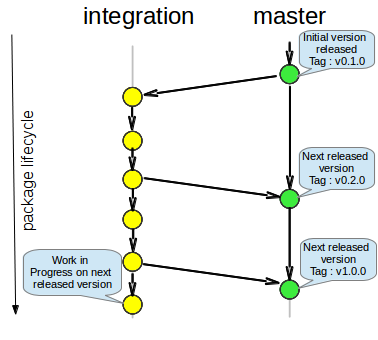
\includegraphics[scale=1]{images/permanent_branches.png}
\caption{Permanent branches of a package}
\label{fig-perm-branches}
\end{figure}

\begin{figure}
\center
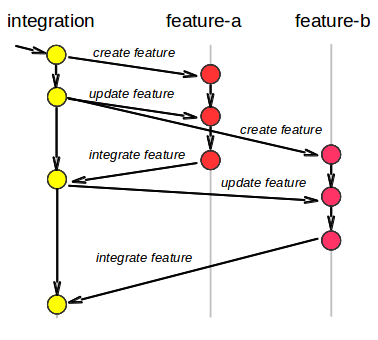
\includegraphics[scale=1]{images/feature_branching.png}
\caption{Relation between feature and integration branches}
\label{fig-feature-branches}
\end{figure}

\textbf{Supporting branches} are temporary branches, used to aid parallel development between team members, ease tracking of features and to assist in quickly fixing live production problems.
\begin{itemize}
\item \textbf{Features} branches (see figure ~\ref{fig-feature-branches}) are used to develop new features /address new topics for the upcoming or a distant future release. Each feature branch must branch from the \textbf{integration} branch. A feature branch exists as long as the feature is in development, but will be merged back into develop (to definitely add the new feature to the upcoming release) or discarded (in case of a disappointing experiment). During its lifetime a feature should be updated from time to time with the modifications contained in the \textbf{integration} branch (issued for instance from the integration of other features). Doing so, the final merge of the feature will be more easy as the state of the feature will be not to far, in terms of importance of modifications, from the state of the \textbf{integration} branch.
\item \textbf{Hotfixes} branches (see figure ~\ref{fig-hotfix-branches}) arise from the necessity to act immediately upon an undesired state of a released version. When a critical bug in a realease version must be resolved immediately, a hotfix branch may be branched off from the corresponding tag on the \textbf{master} branch that marks the production version. Hotfix branches are used to allow team members to continue their work (on the \textbf{integration} and \textbf{feature} branches), while another person is preparing a quick bug/security fix. When bugs are solved, the bug fix must be merged back into both \textbf{master} and \textbf{integration} branches. When merged the \textbf{master} branch is tagged with a new \textit{patch version number}.
\end{itemize}

\begin{figure}
\center
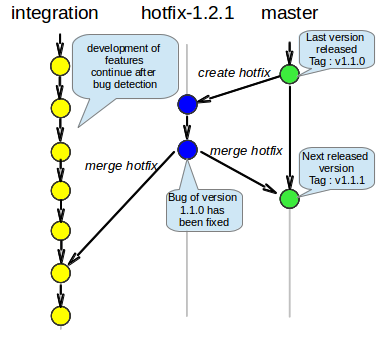
\includegraphics[scale=1]{images/hotfix_branching.png}
\caption{Relation between hotfix and integration/master branches}
\label{fig-hotfix-branches}
\end{figure}

\textbf{Naming Conventions:}
\begin{itemize}
\item a \textbf{feature} branch name starts with "feature-" and ends with the name of the feature (given by developer).
\linebreak example : \texttt{feature-newfunctionnality}
\item a \textbf{hotfix} branch name starts with "hotfix-" and ends with the new \textit{patch version} of the released version.
\linebreak example : \texttt{hotfix-1.2.1}
\end{itemize}

\paragraph{Collaborative working with GIT repositories}

Now that the way the package is structured and is evolving the last part of this section consist in defining how people involved in the package's life cycle work together. The first concern is to define the \textbf{privileges} owned by these persons as regard of the repository usage. To do so we first define the three roles associated to each package:
\begin{itemize}
\item \textbf{users} are people using the package but not involved in its development.
\item \textbf{developers} are users involved in the development of a package.
\item \textbf{administrators} are developers with additional privileges, as they are considered as responsible of the package by users of the package.
\end{itemize}

Privileges associated to each role are managed inside the \textbf{package server} that hosts the package: 
\begin{itemize}
\item each package repository is associated to three \textit{groups}, each one representing a role previously defined. For example, for a package "a-pack" , there are groups "a-pack-users", "a-pack-developers" and "a-pack-administrators". Each group provides specific privileges on the package repository.
\item users registered inside the \textbf{package server} may be affected to one of these \textit{groups}. Doing so, these users obtain corresponding privileges on the package repository.
\item the repository can be set "public" so that anyone is considered as a user. In this case the users group may be not useful and can be let undefined.
\end{itemize}

\begin{figure}
\center
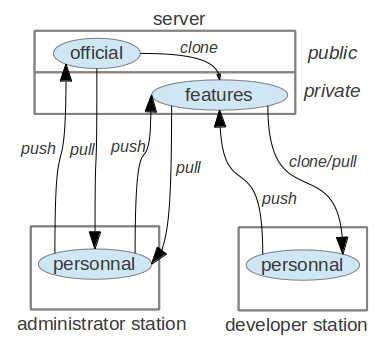
\includegraphics[scale=1]{images/collaborativework.png}
\caption{Collaboration between developers and repository}
\label{fig-collab}
\end{figure}

The basic scheme for collaborative working between package developers is presented in figure~\ref{fig-collab}. 
Given a package, this package has an \textbf{official GIT repository} that is deployed on a given \textbf{package server}. This repository is \textit{official} because it centralizes information of the package and is public, which means that all concerned people (team, laboratory or more generally anyone registered in the server) can access to it. The access in itself is restricted with respects to roles:
\begin{itemize}
\item registered \textbf{administrators} have read/write access on the official package.
\item all other registered \textbf{users} have read access.
\item unregistered people may have read access (i.e. open source repository).
\end{itemize}

During development, one or more \textbf{private repositories} of the package can be created by \textit{forking} the official repository. Depending on the official repository either only registered administrators (private package), developers (protected package), users (public package), or anyone (open package) can \textit{fork} the official repository. Then the creator in addition of the administrators of the official, become \textbf{administrators} of the private repository. Then they can register new \textbf{users} and \textbf{developers} for this repository, with following privileges:
\begin{itemize}
\item registered \textbf{administrators} and \textbf{developers} have read/write access.
\item registered \textbf{users} have read access.
\item unregistered people have no access.
\end{itemize}

These repositories help structuring the development process by grouping developers work around a common repository while not immediately impacting the official one. This lets the time to the \textbf{administrators} to check if everything is OK and that modifications can be merged back into the official repository. The main purpose when using \textbf{private repositories}, is to separate the work on the same package made by different groups. For instance, a PhD student working on its demos on one side and a team with external people working in a common research project on the other side.

Administrators of the official package are the only ones that can update the \textbf{official repository} with modifications made on private repositories. That is why they are responsible of \textit{version releasing} (see previous section): they check the work done by developers and decides if the code is stable enough to release it. Furthermore, if there are many private repositories of the same package they act as brokers of changes made in separate pools of developers.

\subsection{Workspace}

The workspace is the place where developers work with packages (either those they develop or those they simply use). Technically, workspaces are local folder hierarchies in any station (server/demo/developers computers) that works with PID packages. A workspace is the place where packages repositories are created, developed and installed, and referenced given a predetermined pattern. As compared to classical "do as you wish" installation, the workspace notion as several advantages :
\begin{itemize}
\item there is a reference path in the deploy process in such a way that classifying and finding software artefacts is made easy.
\item there is no need to use system dependencies intensively for developed packages. As far as possible, every dependency should be satisfied by workspace content, except for system dependencies that cannot be packaged into workspace.
\item developers can handle many version of a package in the same build/execution environment, without risking to break OS dependencies. Furthermore they can used multiple versions of the same package in the same time.
\end{itemize}

\subsubsection{Workspace organization}

A workspace is a folder (preferably named "workspace") with the following structure:
\begin{itemize}
\item the \textbf{.git} folder contains version control related information, managed by the git tool.

\item the \textbf{install} folder contains packages' binaries installed by the user. 
\item the \textbf{packages} folder contains all the packages developed by an author. Each sub-folder of \textbf{packages} is a local repository of a given package as presented previously.
\item the \textbf{external} folder contains all the external packages used by the installed package (source or binary). Each subdirectory corresponds to an external package, whose content is in turn completely undefined.
\item the \textbf{.gitignore} file is used to exclude  \textbf{install}, \textbf{packages} and \textbf{external} folders content from version control. This is mandatory since these folders content is supposed to be \textbf{ purely local a a user workstation}.
\item the \textbf{share} folder contains important files used to manage packages. The \textbf{docs} sub-folder contains documentation including the present document ; the \textbf{cmake} folder contains all scripts and data required to describe, build, install, deploy and configure packages: the \textbf{find} sub-folder contains cmake find script for commonly used external packages ; the \textbf{system} sub-folder contains generic scripts ; \textbf{patterns} contains cmake pattern files used ; \textbf{references} contains cmake script files with meta-information about available packages ; \textbf{licenses} contains cmake script files containing available license description; 
\end{itemize}


The install folder contains installed binary version(s) of any package used by a user. Each of its direct sub directories is a folder representing a given installed package, that itself contains :
\begin{itemize}
\item as many folders as there are concurrent binary versions of the package installed. The name of the version folder reflects the installed package version it contains (e.g. : 1.3.5 ; 1.2.0, etc.). Version folder can be also local (correspond to an install from a source package currently developed in the workspace), in such a case they name is of the form : own-0.2.5, own-1.0.0, etc.)
\item an \textbf{installers} folder that contains all installable binary archives with each archive that corresponds to a specific version, for a specific system (linux, mac), in a specific mode (release, debug).
\end{itemize}

where are installed package binary versions.
 
A framework is a folder (whose name is a given unique package name) contained in the \textbf{frameworks} folder of the workspace. It contain Each version folder is organized according to the following structure. 
\begin{itemize}
\item the \textbf{CMakeModules} folder contains all cmake scripts files (.cmake) used to find and configure required runtime dependencies.
\item the \textbf{bin} folder contains \textbf{release} and \textbf{debug} subdirectories that themselves contain executable/scripts of the package either in debug or release mode.
\item the \textbf{tests} folder contains test executable/scripts of the package placed in \textbf{release} and \textbf{debug} subdirectories according to their build mode.
\item the \textbf{include} folder contains the exported interfaces of libraries, like .h/.hpp files in C/C++. Basically, its direct sub-folders are libraries' root folder hierarchically organized the same way as in the package repository \textbf{include} folder.
\item the \textbf{lib} folder contains \textbf{release} and \textbf{debug} subdirectories that themselves contain libraries of the package either in debug or release mode.
\item the \textbf{config} folder contains all configuration files required by executables (not for tests) or libraries.
\item the \textbf{launch} folder contains launch scripts for executables.
\item the \textbf{share} folder contains documents (e.g. tutorial, design reports, install procedure) including code documentation files or documents (latex) generated by the doxygen tool.
\item the \textbf{license.txt} file describes the license that applies to the software. This is a copy of the license file in package repository.
\item the \textbf{package.manifest} file contains meta-data about the package. It is a simple copy of the same file in package repository for the considered version.
\end{itemize}
There is also a specific version folder in the framework, named \textbf{own}, in which are installed artefacts resulting from the current package in development. A package has to be installed in this specific version folder whenever the developer works on another than \textbf{master branch} (that theoretically contains only released versions).
Finally, the framework also contains a folder named \textbf{installers} in which are placed all OS installers for all version and target platforms that have been generated by a developer or that have been used to deploy a given package version.



\subsubsection{Workspace repository}

The \textbf{official workspace} is a git repository that can be modified only by \textbf{administrators} of the server. It contains cmake scripts used notably to:
\begin{itemize}
\item reference available packages (repositories and binary archives). Each time a new package is created it is referenced into the local workspace (by an administrator) and then changes in the official workspace are committed so that anyone can know the existence of this new package and can retrieve its hosting server. This does not mean that this person can use binary version or repository of this package, since this is bound to his access rights to the servers (at least one can know which person to call to get the rights).
\item provide available licenses description. These descriptions will be used in packages description.
\end{itemize}

The \textbf{official workspace} can be forked into \textbf{private workspaces}, exactly the same way as an \textbf{official package} (see figure~\ref{fig-collab}), to provide a common workspace for a team developing one or more packages at the same time. Once created new \textbf{users} and \textbf{developers} can be added to the private workspace repository. Private workspaces will be updated (by \textbf{developers} and \textbf{administrators}) with new references to packages, new licenses and new find scripts, while new packages are implemented. Then \textbf{official workspace} administrators can update its content, at any time, with the modifications made inside the private repository.

\pagebreak

\section{Work-flow}

Now that all basic concepts and principles have been described, this last section shows how to use them during the development process.

\subsection{Installing Workspace and Packages}

The first phase when starting development consists in installing a workspace on the local  station of a developer or administrator, and configuring it adequately.

\subsubsection{Getting Last Workspace Version}

This phase simply consists in cloning the workspace repository. Any member of the robotic department can clone this repository, but only administrators can  modify it.

\begin{verbatim}
	git clone <global account>@<official server>:workspace.git
\end{verbatim}

When done the developer can start his work. The workspace is empty, which means it only contains available licenses description in \textbf{licenses} folder, references to available packages in \textbf{references} folder, generic package structure in \textbf{patterns} folder, \textbf{CMakeModules} folder with existing cmake scripts and a complete \textbf{categories} folder with links that target nothing. Its \textbf{packages} and \textbf{frameworks} are empty.

We have to notice that only \textbf{administrators} have direct write access to the official servers and developers may or not have read access. Consequently, developers cannot modify the workspace repository.
 
\subsubsection{Starting Development}

Then the \textbf{developer} has two choices:
\begin{itemize}
\item either he starts the development of a new package,
\item or he starts working on an existing package.
\end{itemize}

\paragraph{When a new package is created:}
\begin{enumerate}
\item an \textbf{administrator} creates an empty GIT repository and optionally an associated (sub)project (e.g. a \textit{redmine} project) on a given server (team or laboratory or open).
\item the \textbf{administrator} initializes the repository. On his local station he does:
\linebreak \verb|cd <workspace path>/packages/|
\linebreak \verb|git clone <global account>@<official server address>:<new package>.git|
\linebreak \verb|cd <new package>|
\linebreak \verb|cp -R ../../../patterns/package/ .|
\linebreak \verb|git tag -a v0.0.0 -m "creation of package"|
\linebreak \verb|git checkout -b develop master|
\linebreak \verb|git commit -a -m "initialization of package done"|
\linebreak \verb|git push origin master|
\linebreak \verb|git push origin develop|
\item the \textbf{administrator} creates a private account on the same or another server (or uses an existing one) and he clones the new repository in this account:
\linebreak \verb|git clone <global account>@<official server address>:<new package>.git|
\linebreak \verb|cd <new package>|
\item the \textbf{administrator} creates \textbf{feature branches} on private repository, by doing:
\linebreak \verb|git checkout -b feature-<feature name> develop|
\item the \textbf{administrator} registers the new developer (and any other person that may be involved in the development of this package) with ssh, so that he can access the git repository.
\item now \textbf{developers} can update/work with the private repository as they wish. To do this on their local working station they do :
\linebreak \verb|cd <workspace path>/packages/|
\linebreak \verb|git clone <private account>@<any server address>:<new package>.git|
\end{enumerate}

When done the development can start inside a package that is generic: it contains only the folder hierarchy and pattern files (e.g. doxyfile, CMakeList.txt, package.manifest, .gitignore) that matches the package structure defined in section 1.

\paragraph{When the developer start working on an existing package:} 
He either works on existing features or on new features. In the first case the \textbf{administrator} simply has to register the \textbf{developer} on the existing private server (step 5-6). In the second case, the administrator has to choose:
\begin{itemize}
\item if a new private repository has to be created, for instance, in order to isolate the work made on new branches (steps 3 to 6).
\item or if the developer uses an existing private repository with new branches (steps 4 to 6).
\end{itemize}
 
Whatever the solution chosen, the development starts in a package that already  contains some specific software artefacts and has "generic files" already configured. The developer may then need to install new existing packages.

\subsubsection{Installing Required Packages in the Workspace}

When starting development with an existing package, this later can have one or more dependencies with another packages and with system. System dependencies must be fulfil using classical install process provided by the OS. They can be found when compiling the package for the first time with \textbf{cmake}. Package dependencies are managed in another way:
\begin{enumerate}
\item to know which package are required, the developer has to look at the \textbf{package.manifest} file. The \texttt{dependency} markups list the required packages.
\item then the developer has to download and install these packages in its local workspace. To do so there are some alternatives:
\begin{itemize}
\item the developer has a \textbf{read access} to the official repository of the package (it is listed in the corresponding \texttt{dependency} markup). In this case he can simply do:
\linebreak \verb|cd <workspace path>/packages/|
\linebreak \verb|git clone <global account>@<official server>:<other package>.git|
\linebreak \verb|cd <other package>|
\linebreak \verb|git checkout tags/v<version compatible with requirements>|
\linebreak \verb|cd build|
\linebreak \verb|cmake ..|
\linebreak \verb|make|
\linebreak \verb|make install|
\item The developer can take a look at the \texttt{<package name>.manifest} file in the \textbf{references} folder of the workspace to know if there are installers available and if they match the required version. In this case, the developer uses the OS installer system and target the required package framework. For instance, for a package that is a simple archive :
\linebreak \verb|cd <workspace path>/frameworks/|
\linebreak \verb|ftp ftp://ftp.gforge.fr/<other package>-<version>.tgz|
\linebreak \verb|tar -xzvf <other package>-<version>.tar.gz|
\end{itemize}
\item When the last operation has been repeated for all packages, the frameworks of all packages contain adequate versions. Direct dependencies are resolved, but these required packages can in turn require other packages and OS dependencies. The current procedure has to be repeated recursively for each of these indirectly required packages.
\end{enumerate}

Once all the dependencies are satisfied, the development can truly start.

\subsection{Collaborative Software Development}

All \textbf{developers} only work around \textbf{private repositories} of packages, while \textbf{administrators} are responsible of the update of \textbf{official repositories} according to the changes done in private repositories. Nearly all developments in \textbf{private repositories} are made in \textbf{feature branches}. The \textbf{develop branch} is used to merge and to solve conflict between features.

\subsubsection{Developing a Feature}

Common feature branches are already created, so the only thing to do for developers is to navigate between available feature branches and add content in branches :
\begin{itemize}
\item Each time a developer wants to start making modification of a given feature (for instance at the beginning of the day):
\linebreak \verb|git checkout feature-<feature name>|
\linebreak \verb|git pull origin feature-<feature name>|
\linebreak \verb|=> solving potential conflicts|
\item During development of a feature, developers need to frequently "save" their work locally:
\linebreak \verb|git add <modified files>|
\linebreak \verb|git commit -m "<telling modifications>"|
\item Each time a developer wants to stop making modification of a given feature (for instance at the end of the day) or when important modification have been finished and committed:
\linebreak \verb|git pull origin feature-<feature name>|
\linebreak \verb|=> solving potential conflicts|
\linebreak \verb|git push origin feature-<feature name>|
\end{itemize}

During development on a feature branch, a developer may need to test some ideas without disrupting the work of all people working on the feature. In that case, he can work with a \textbf{new local branch} forked from feature branch. Modifications in this branch stay always local to the developer station. Furthermore modification should not be too big, these branches are used to test some ideas or to do bug fixes, not for developing big features (this is the role of feature branches) !
\begin{itemize}
\item Creating a local branch for testing an idea :
\linebreak \verb|git checkout feature-<feature name>|
\linebreak \verb|git pull origin feature-<feature name>|
\linebreak \verb|=> solving potential conflicts and testing|
\linebreak \verb|git push origin feature-<feature name>|
\linebreak \verb|git checkout -b <idea name> feature-<feature name>|
\item During development of the idea, frequently save the work locally:
\linebreak \verb|git add <all files modified>|
\linebreak \verb|git commit -m "<telling modifications>"|
\item When idea is OK and can be integrated to the feature:
\linebreak \verb|git pull origin/feature-<feature name>|
\linebreak \verb|=> solving potential conflicts and testing|
\linebreak \verb|git rebase origin/feature-<feature name>|
\linebreak \verb|git checkout feature-<feature name>|
\linebreak \verb|git merge <idea>|
\linebreak \verb|git branch -d <idea>|
\linebreak \verb|git push origin feature-<feature name>|
\item otherwise if the idea is not good:
\linebreak \verb|git checkout feature-<feature name>|
\linebreak \verb|git branch -d <idea>|
\end{itemize}

The idea behind the use of the rebase command is to let the history of the feature development as linear as possible, in order to 

\subsubsection{Integrating Features}

During development process, features have to be incrementally integrated as soon as their development is finished and they have been tested. The integration can be done either by developers or administrators, but in all cases it requires every developers of the feature to be aware of this, to avoid big troubles.
\begin{enumerate}
\item Merging the feature in the development branch:
\linebreak \verb|git checkout feature-<feature name>|
\linebreak \verb|git pull origin develop|
\linebreak \verb|=> solving conflicts and testing|
\linebreak \verb|git checkout develop|
\linebreak \verb|git merge --no-ff feature-<feature name>|
\linebreak \verb|=> solving conflicts and testing|
\item Deleting the feature branch:
\linebreak \verb|git push origin develop|
\linebreak \verb|git push origin --delete feature-<feature name>|
\item Updating in local repository the branch that has been removed in remote repository (all users of the repository) :
\linebreak \verb|git remote prune origin|
\linebreak \verb|git branch -d feature-<feature name>|
\end{enumerate} 

\paragraph{Remarks:}
\begin{itemize}
\item The development of features is made in parallel and they are merged indirectly in the \textbf{develop branch} at the very end, one at a time: features don't synchronize until merge. This let the possibility to developers to change some parts of the API/structure without immediately impacting the work made on others features.
\item The best way is to first create an initial feature branch that puts in place the general basis of the package (API, basic class hierarchy, etc.). Then, when this feature has been merged in develop branch, parallel development into many feature branches can start.
\item When merging, the resolution of conflicts \textbf{must be realized in feature branch} to avoid any problem in the develop branch while conflicts resolution take place.
\end{itemize}

\subsubsection{Releasing a Package Version}

Releasing package versions is the responsibility of administrators.

The first step is the update of the administrator station with modifications contained in private repository (named \texttt{private}):
\begin{enumerate}
\item Merging develop into master:
\linebreak \verb|git checkout develop|
\linebreak \verb|git pull private develop|
\linebreak \verb|git checkout master|
\linebreak \verb|git merge --no-ff develop|
\linebreak \verb|doing test and solving conflicts, if any|
\linebreak Incrementing the version number in \textbf{package.manifest} file to get \texttt{<new version number>}.
\linebreak \verb|git commit -a -m "Bumped version to <new version number>"|
\linebreak \verb|git tag -a v<new version number>|
\item Updating private repository with new release version (to simply update the \textbf{package.manifest} file):
\linebreak \verb|git checkout develop|
\linebreak Incrementing the version number in \textbf{package.manifest} file to get \texttt{<new version number>}.
\linebreak \verb|git commit -a -m "Bumped version to <new version number>"|
\linebreak \verb|git push private develop|
\linebreak \verb|git push private master|
\end{enumerate}

The second step consists in updating the official repository (named \texttt{origin} for the administrator):
\begin{enumerate}
\item Getting branches from official repository:
\linebreak \verb|git checkout develop|
\linebreak \verb|git pull origin develop|
\linebreak \verb|doing test and solving conflicts, if any|
\linebreak \verb|git checkout master|
\linebreak \verb|git pull origin master|
\linebreak \verb|doing test and solving conflicts, if any|
\item Update the master and develop branches:
\linebreak \verb|git push origin develop|
\linebreak \verb|git push origin master|
\end{enumerate}


\subsubsection{Developing a Hotfix}

Creating a hot fix is always made on demand of an administrator, but can be realized either by himself or a developer. The process is quite the same as for features, but we suppose that only one developer is involved in this task, that should be quick: 
\begin{enumerate}
\item a package private repository is created or an existing one is used.
\item The administrator gets the last released version number from \textbf{package.manifest} file (e.g. 1.2.0) and increments the patch version number to get the <new patch version number> (e.g. 1.2.1).
\item Creating the hotfix branch in the private repository:
\linebreak  \verb|git checkout -b hotfix-<new patch version number> master|
\item During the bug correction, committing locally:
\linebreak \verb|git checkout hotfix-<new patch version number>|
\linebreak \verb|git add <modified files>|
\linebreak \verb|git commit -m "<commit message>"|
\item Saving work in the private repository:
\linebreak \verb|git push origin hotfix-<new patch version number>|
\end{enumerate}

When bug or security problems have been solved and tested, the development of the hotfix is finished. This is then the only time when the master branch can be modified in the private repository:
\begin{enumerate}
\item The responsible of the hotfix releases it:
\linebreak \verb|git checkout hotfix-<new patch version number>|
\linebreak \verb|changing version number is package.manifest file|
\linebreak \verb|git commit -a -m "Bumped version to <new patch version number>"|
\linebreak \verb|git checkout master|
\linebreak \verb|git merge --no-ff hotfix-<new patch version number>|
\linebreak \verb|git tag -a v<new patch version number>|
\linebreak \verb|git push origin master|
\linebreak \verb|git checkout develop|
\linebreak \verb|git merge --no-ff hotfix-<new patch version number>|
\linebreak \verb|doing some conflicts resolution if necessary|
\linebreak \verb|git push origin develop|
\item Then the hotfix branch is deleted:
\linebreak \verb|git branch -d hotfix-<new patch version number>|
\linebreak \verb|git push origin --delete hotfix-<new patch version number>|
\end{enumerate}

Then the last step consists in releasing the patch version on the official server. This is the role of administrators that do that on their own station:
\begin{enumerate}
\item Updating master and develop branches:
\linebreak \verb|git pull private develop|
\linebreak \verb|git pull private master|
\item Checking that the hotfix solves the problem and that everything is OK.
\item Updating official repository branches:
\linebreak \verb|git push origin develop|
\linebreak \verb|git push origin master|
\end{enumerate}


\subsection{Updating workspace}

Updating the workspace repository must be done:
\begin{itemize}
\item when a new package has been created and first released version has been published on package official server: the \textbf{package.manifest} file must be added  and renamed to the \textbf{references} folder of the workspace.
\item when a new version of an existing package has been release on a package official server: the corresponding \textbf{package.manifest} in the the \textbf{references} folder of the workspace must be updated.
\item when a new license is used in a \textbf{package.manifest} file: the corresponding license file must be added to the \textbf{licenses} folder of the workspace.
\item when categories defined in a \textbf{package.manifest} file have changed: the folders for new (sub)categories have to be created ; the link to the package framework have to be created or suppressed (when the package has been removed from a category).
\item when a new package is released on official server and it targets some categories: links to that packages have to be added to target (sub)categories folders.
\end{itemize}
 
The update of the workspace is the work of the \textbf{administrators} only: they are responsible to guarantee the coherence of workspace repository structure and content.

\subsubsection{Adding references to packages}

When a package is added to the workspace official repository, on its local workstation an administrator of the package does:
\begin{enumerate}
\item Referencing the package in the workspace:
\linebreak \verb|cd <path to the package>|
\linebreak \verb|git pull origin master|
\linebreak \verb|git checkout master|
\linebreak \verb|cp package.manifest ../../references/<nameofpackage>.manifest|
\linebreak \verb|git commit -a -m "adding package <package name>"|
\item Looking package license in \textbf{package.manifest} and if the license does not exists in workspace create the corresponding license file:
\linebreak \verb|cd <path to the workspace>|
\linebreak \verb|cp patterns/license.license licenses/<licensename>.license|
\linebreak \verb|writing the new license file...|
\linebreak \verb|git commit -a -m "adding license <license name>"|
\item Looking package categories in \textbf{package.manifest} file, and if categories do not exist, create them:
\linebreak \verb|cd <path to the workspace>/categories|
\linebreak \verb|mkdir <category path>|
\linebreak \verb|git commit -a -m "adding category <category name>"|
\item Adding a link to the package framework in each category folder defined in \textbf{package.manifest} file:
\linebreak \verb|cd <path to the workspace>/<path to category folder>|
\linebreak \verb|ln -s -t . <relative path to workspace root>/frameworks/<package name>|
\linebreak \verb|git commit -a -m "adding link to <package> in <category name>"|
\item If a package requires some system dependencies that the administrator think to be relevant for many developers, he can add the cmake script files used to configure these dependencies to the \textbf{CMakeModules} folder of the workspace.
\linebreak \verb|cd <path to the workspace>/CMakeModules|
\linebreak \verb|cp <path to the workspace>/packages/<name of package>/|
\linebreak \verb| CMakeModules/<chosen dependency>.cmake .|
\linebreak \verb|git commit -a -m "adding cmake script for <dependency>"|
\item Updating the workspace official repository:
\linebreak \verb|cd <path to the workspace>|
\linebreak \verb|git pull origin master|
\linebreak \verb|solving potential conflicts|
\linebreak \verb|git push origin master|
\end{enumerate}

\subsubsection{Removing references to packages}

The process is quite the same as previously except that only the package reference file is suppressed from the workspace references folder, not the license files or the categories.
\begin{enumerate}
\item Removing the package reference:
\linebreak \verb|cd <path to the workspace>/references|
\linebreak \verb|rm <package name>.manifest|
\linebreak \verb|git commit -a -m "removing package <package name>"|
\item Updating the workspace official repository:
\linebreak \verb|cd <path to the workspace>|
\linebreak \verb|git pull origin master|
\linebreak \verb|solving potential conflicts|
\linebreak \verb|git push origin master|
\end{enumerate}

\subsubsection{Updating references to packages}

The update of a package reference must be done \textbf{each time a new version of the package is released} in the official repository of the package. The process is the same as for adding the package reference for the first time, except for categories:

\begin{enumerate}
\item Looking package categories in the new version of the \textbf{package.manifest} file, and if categories do not exist, create them:
\linebreak \verb|cd <path to the workspace>/categories|
\linebreak \verb|mkdir <category path>|
\linebreak \verb|git commit -a -m "adding category <category name>"|
\item Adding a link to the package framework in each category folder defined in \textbf{package.manifest} file:
\linebreak \verb|cd <path to the workspace>/<path to category folder>|
\linebreak \verb|ln -s -t . <relative path to workspace root>/frameworks/<package name>|
\linebreak \verb|git commit -a -m "adding link to <package> in <category name>"|
\item Removing links in each category folder no more defined in \textbf{package.manifest} file:
\linebreak \verb|rm <path to the workspace>/<path to old category folder>/<package name>|
\item Updating the workspace official repository:
\linebreak \verb|cd <path to the workspace>|
\linebreak \verb|git pull origin master|
\linebreak \verb|solving potential conflicts|
\linebreak \verb|git push origin master|
\end{enumerate}

\pagebreak
\section{Project Management with CMake}

During development, developers have to handle many types of files. While package.manifest files are mainly managed by administrators, files used to build/install/test and generate documentation are mainly written by developers. This section focuses on the usage of these files and good practices to follow.

CMake is the reference tool to manage the development process in a package. The CMakeFile.txt script describes how the package is built, tested, installed, packaged into an OS installer, and how its documentation is generated. A basic pattern of CMakeList.txt is provided in the workspace and explanations are given in following subsections:

\subsection{Header of the root CMakeList.txt file}

The beginning of the file looks like this:

\begin{verbatim}
PROJECT(<package name>)
CMAKE_MINIMUM_REQUIRED(VERSION 2.8)

# generic variables
set(FRAMEWORKS_DIR ${CMAKE_SOURCE_DIR}/../../frameworks)
set(FRAMEWORK_PATH ${FRAMEWORKS_DIR}/${PROJECT_NAME})

# setting the current version number
set (${PROJECT_NAME}_VERSION_MAJOR <major number>)
set (${PROJECT_NAME}_VERSION_MINOR <minor number>)
set (${PROJECT_NAME}_VERSION_PATCH <patch number>)
set(${PROJECT_NAME}_VERSION  ${${PROJECT_NAME}_VERSION_MAJOR}.
${${PROJECT_NAME}_VERSION_MINOR}.${${PROJECT_NAME}_VERSION_PATCH}

# basic build options
option(${PROJECT_NAME}_WITH_EXAMPLES "Package build examples" ON)
option(${PROJECT_NAME}_WITH_TESTS "Package uses tests" ON)
option(USE_CUSTOM_DEPLOYMENT "deploying in own folder of the framework
instead of the version folder" ON)

# setting the current version number
set (${PROJECT_NAME}_VERSION_MAJOR 0)
set (${PROJECT_NAME}_VERSION_MINOR 1)
set (${PROJECT_NAME}_VERSION_PATCH 0)
set(${PROJECT_NAME}_VERSION ${${PROJECT_NAME}_VERSION_MAJOR}
.${${PROJECT_NAME}_VERSION_MINOR}.${${PROJECT_NAME}_VERSION_PATCH})

# configuring installation process into frameworks: by default
# version specific deployment is selected except if users define
# USE_LOCAL_DEPLOYMENT variable

# just use the option USE STANDARD DEPLOYMENT if you want to install 
# in basic install folmders (e.g. /usr/local/include, /usr/local/lib 
# and /usr/local/bin) 
option(USE_STANDARD_DEPLOYMENT "Package uses standard deployment rules" OFF)
if (USE_STANDARD_DEPLOYMENT)
message("Deployment : standard deployment ...")
else(USE_STANDARD_DEPLOYMENT)
option(USE_LOCAL_DEPLOYMENT "Package uses tests" ON)
if(USE_LOCAL_DEPLOYMENT)
MESSAGE("Deployment : package is deployed in the own folder of its framework")
set(DEPLOY_PATH own)
else(USE_LOCAL_DEPLOYMENT)
MESSAGE("Deployment : package is deployed in the version folder 
 ${${PROJECT_NAME}_VERSION} of its framework")
set(DEPLOY_PATH ${${PROJECT_NAME}_VERSION})
endif(USE_LOCAL_DEPLOYMENT)
set(CMAKE_INSTALL_PREFIX ${FRAMEWORK_PATH})
endif(USE_STANDARD_DEPLOYMENT)

# adding the cmake scripts files from the package 
# and from the workspace
list(APPEND CMAKE_MODULE_PATH ${CMAKE_SOURCE_DIR}/CMakeModules)
if (NOT USE_STANDARD_DEPLOYMENT)
list(APPEND CMAKE_MODULE_PATH /../../CMakeModules)
endif(NOT USE_STANDARD_DEPLOYMENT)
#otherwise cmake scripts must be insalled else where (default folder)

\end{verbatim}

First part defines the general settings of the project that should be quite the same for all packages:
\begin{itemize}
\item name of the cmake project is the name of the package.
\item basic options for package users/developers are set in order to let the possibility to build examples and test units (i.e. non functional code).
\item version number matches the current version number of the package. it \textbf{must be updated each time a new release version is tagged on master branch}.
\item if a user defines the \verb|USE_CUSTOM_DEPLOYMENT| variable, the deployment of the package in framework will be done in the \textbf{own} folder and not in the \textbf{version} folder.
\item directories containing cmake script files used (e.g. to find os dependencies) are referenced in the \verb|CMAKE_MODULE_PATH| variable. 
\end{itemize}

\subsection{Managing system dependencies}

The next step consists in finding/configuring system dependencies for the package. Fortunately, CMake provides a standard way to do that using the \verb|find_package| command. This command helps finding resources installed in the system and get useful information about the dependency: it calls a specific cmake script (whose pattern name is \texttt{Find<name of package or library>.cmake}) that is able to do the job.

Here is the way we use the \verb|find_package| command:

\begin{verbatim}
##### finding system dependencies #####
SET(EXTERNAL_INCLUDE_DIRS "")
SET(EXTERNAL_LIB_DIRS "")
SET(EXTERNAL_LIBS "")
SET(EXTERNAL_APPS "")
SET(EXTERNAL_APP_DIRS "")

## absolutely required dependencies ##
find_package(<name of resource> REQUIRED)
list(APPEND EXTERNAL_INCLUDE_DIRS ${<name of resource>_INCLUDE_DIRS})
list(APPEND EXTERNAL_LIB_DIRS ${<name of resource>_LINK_DIRECTORIES})

## optional system dependencies ##
find_package(<name of resource 4>)
if(<name of resource 4>_FOUND)
option(USE_<name of resource 4> "Using <name of resource 4>" ON)
else(<name of resource 4>_FOUND)
set (USE_<name of resource 4> FALSE)
endif(<name of resource>_FOUND)
if(USE_<name of resource 4>)
list(APPEND EXTERNAL_INCLUDE_DIRS ${<resource 4_INCLUDE_DIRS>})
list(APPEND EXTERNAL_LIB_DIRS ${<resource 4_LINK_DIRECTORIES>})
add_definitions(-DUSE_<name of resource 4>)
endif(USE_<name of resource 4>)
...

## alternatively required system dependencies ##
# defining alternative 1
find_package(<name of resource 2>)
if(<name of resource 2>_FOUND)
option(USE_<name of resource2> "Using <name of resource2>" ON)
else(<name of resource 2>_FOUND)
set(USE_<name of resource2> FALSE)
endif(<name of resource 2>_FOUND)
# defining alternative 2
find_package(<name of resource 3>)
if(<name of resource 3>_FOUND)
option(USE_<name of resource3> "Using <name of resource3>" ON)
else(<name of resource 3>_FOUND)
set(USE_<name of resource 3> FALSE)
endif(<name of resource 3>_FOUND)

# selecting the alternative
if(USE_<name of resource 2>)
list(APPEND EXTERNAL_INCLUDE_DIRS ${<resource 2_INCLUDE_DIRS>})
list(APPEND EXTERNAL_LIB_DIRS ${<resource 2_LINK_DIRECTORIES>})
add_definitions(-DUSE_<name of resource 2>)
elseif(USE_<name of resource 3>)
list(APPEND EXTERNAL_INCLUDE_DIRS ${<resource 3_INCLUDE_DIRS>})
list(APPEND EXTERNAL_LIB_DIRS ${<resource 3_LINK_DIRECTORIES>})
add_definitions(-DUSE_<name of resource 3>)
else(USE_<name of resource 2>)
MESSAGE("alternative system dependency not satisfied. Install/select either 
<name of resource 2>, <name of resource 3> or <name of resource 4>")
return()
endif(USE_<name of resource 2>)
...
##### end finding system dependencies #####

\end{verbatim}

There are mainly three way to manage system dependencies, all of them relying on the \verb|find_package| command or one of its derivative (e.g. like \verb|find_library|) or one of its options (e.g. \verb|VERSION| constraints):
\begin{itemize}
\item On way is to require a system dependency using \verb|find_package| with the \verb|REQUIRED| argument. That means that the dependency is absolutely required and the build process will stop if it is not satisfied. This is \textbf{the preferred way to manage dependencies} as it defines clear dependencies between the package and some resources: whatever the OS on which it is deployed, the package will have the same dependency. Of course this is not always possible because it supposes that the required system dependency (e.g. library) exists on all target platforms of the package. This for instance the case for \textbf{boost}.
\item Another way is to define \textbf{optional system dependencies}. This way, the argument \verb|REQUIRED| is not used: if the resource is found, then the option to use it or not is provided to the user, otherwise it cannot be used in any way.  There is a restriction on the use of optional dependencies for the functional code: \textbf{the code that uses them must work even if they are not satisfied}. In other words, the developers have implemented a way to provide same functionalities (certainly in a less optimized or more verbose way) with or without using these optional dependencies. 
\item By extension of the optional dependencies, developers can also use \textbf{alternative system dependencies}, that work quite the same way, except that \textbf{many packages can be selected by users but only one will be used by the build process}. This is not the preferred way but may be mandatory when dealing with libraries that are intrinsically bound to OS or when optimization becomes a major concern (e.g. 2D/3D graphics). In that case all options whose package are selectable and they have strict selection priorities (manages via a simple \verb|if|).
\end{itemize} 

When a system dependency is satisfied, whatever its nature (required, optional, alternative), all its relative system resources have to be included  in the project. To do so we use variables provided by cmake scripts in order to configure:
\begin{itemize}
\item path to libraries.
\item name of libraries.
\item path to header files of libraries.
\end{itemize}
\paragraph{Remarks:}
\begin{itemize}
\item cmake script file behaviours are quite different from each other and consequently names of their output variables and which kind of resources they target differ.
\item of course any other kind of resource than libraries, as soon as they are provided by cmake script files, can be imported in the cmake project, but libraries are the far most common ones.
\item In a package we have to dissociate the optional code from the rest of the functional code. System dependencies for optional code follow exactly the same pattern has described above but they are guarded with respective options variables \texttt{<package>\_WITH\_EXAMPLES} and \texttt{<package>\_WITH\_TESTS}, for instance:
\end{itemize}

\begin{verbatim}
if(<package>_WITH_EXAMPLES)
# defining required, optional or alternative system dependency
# for examples executables
...
endif(<package>_WITH_EXAMPLES)
\end{verbatim}

\subsection{Managing package dependencies}

Package dependencies are different from system dependencies in some ways:
\begin{itemize}
\item \textbf{required packages are absolutely mandatory}, there is no possible option or alternative. 
\item they follow a unified and cross platform installation process, which allows to generically find and use them in an unified way.
\end{itemize} 

Here is the example of a package that requires two other packages:
\begin{verbatim}
# searching for package dependencies
find_package(FrameworkFinder REQUIRED COMPONENTS <package 1> <package 2> ...)
list(APPEND EXTERNAL_INCLUDE_DIRS ${<package 1>_INCLUDE_DIRS})
list(APPEND EXTERNAL_LIB_DIRS ${<package 1>_LINK_DIRECTORIES})
list(APPEND EXTERNAL_LIBS ${<package 1>_LIBRARIES})
list(APPEND EXTERNAL_APP_DIRS ${<package 1>_APP_DIRS})
list(APPEND EXTERNAL_APPS ${<package 1>_APPLICATIONS})

list(APPEND EXTERNAL_INCLUDE_DIRS ${<package 2>_INCLUDE_DIRS})
list(APPEND EXTERNAL_LIB_DIRS ${<package 2>_LINK_DIRECTORIES})
list(APPEND EXTERNAL_LIBS ${<package 2>_LIBRARIES})
\end{verbatim}

The idea is nearly the same as for system dependencies, and the same \verb|find_package| command is used. The main difference comes from the cmake script used, called \texttt{FindFrameworkFinder.cmake}, that is a generic script that does the required job: finding packages and configuring adequately variables. 

\subsection{Building sources}

Once external dependencies have been satisfied, the work of the CMakeFile.txt script is to build the sources, do unit tests and install the resulting software in frameworks. This is simply done with:
\begin{verbatim}
# if all dependencies are satisfied
include_directories(include)
include_directories(${EXTERNAL_INCLUDE_DIRS})
link_directories(${EXTERNAL_LIB_DIRS})

set ( INSTALL_LIB_PATH ${DEPLOY_PATH}/lib)
set ( INSTALL_AR_PATH  ${DEPLOY_PATH}/lib)
set ( INSTALL_HEADERS_PATH ${DEPLOY_PATH}/include)
set ( INSTALL_TESTS_PATH ${DEPLOY_PATH}/tests)
set ( INSTALL_CONFIG_PATH ${DEPLOY_PATH}/config)
set ( INSTALL_SHARE_PATH ${DEPLOY_PATH}/share)
set ( INSTALL_BIN_PATH ${DEPLOY_PATH}/bin)
if(CMAKE_BUILD_TYPE MATCHES Release)
set ( INSTALL_PATH_SUFFIX release)
elsif(CMAKE_BUILD_TYPE MATCHES Debug)
set ( INSTALL_PATH_SUFFIX debug)
endif(CMAKE_BUILD_TYPE MATCHES Release)

add_subdirectory(src)
add_subdirectory(apps)
add_subdirectory(test)
add_subdirectory(share)
add_subdirectory(config)
...
\end{verbatim}

Includes files are referenced with the \texttt{include directories} as they will surely be useful for the entire of functional code. Same way, folders containing libraries used are referenced. The remaining of the build process is done in generic subdirectories of the package, using the \texttt{add\_subdirectory()} command.

The \textbf{src} subdirectory contains a CMakeList.txt file that builds libraries. The simpler way is to define the whole build process directly in this file but developers can also refine the build process in subdirectories if it is very complex. Whatever the solution the code should look like this:
\begin{verbatim}
# building sources
## first subdirectory of src: a library ##
set(LIB_SRC_<lib name> "")
list(APPEND LIB_SRC_<lib name> <lib name>/<path to file>)
list(APPEND LIB_SRC_<lib name> <lib name>/<path to file>)
...
add_library(<lib name>_st STATIC LIB_SRC_<lib name>)
target_link_libraries(<lib name>_st EXTERNAL_LIBS)

add_library(<lib name>_sh SHARED LIB_SRC_<lib name>)
target_link_libraries(<lib name>_sh EXTERNAL_LIBS)
## second subdirectory of src: a library ##
...
\end{verbatim}
By default the best solution is to generate a library both in static and shared mode, to let to library users the biggest choice considering their development.

The \textbf{apps} subdirectory contains a CMakeList.txt file that builds applications. The organization into subdirectories follows the same logic as for libraries:
\begin{verbatim}
## first subdirectory of apps: an executable ##
set(EXE_SRC_<exe name> "")
list(APPEND EXE_SRC_<exe name> <exe name>/<path to file>)
list(APPEND EXE_SRC_<exe name> <exe name>/<path to file>)
...
add_executable(<exe name> EXE_SRC_<exe name>)
target_link_libraries(<exe name> <lib name>_st)

if(<package>_WITH_EXAMPLES)
## second subdirectory of apps: an example executable ##
set(EXE_SRC_<exe name> "")
list(APPEND EXE_SRC_<exe name> <exe name>/<path to file>)
list(APPEND EXE_SRC_<exe name> <exe name>/<path to file>)
...
add_executable(<exe name> EXCLUDE_FROM_ALL EXE_SRC_<exe name>)
target_link_libraries(<exe name> <lib name>_sh)
...
## building example targets, if any ##
add_custom_target(examples COMMAND ${CMAKE_COMMAND} -E echo "Building 
examples targets" DEPENDS <example 1> <example 2>...)
endif(<package>_WITH_EXAMPLES)

\end{verbatim}
The main difference with libraries is the usage of the \verb|add_executable| command to create executable and the use of a guard (\verb|if(<package>_WITH_EXAMPLES)|) to avoid building examples applications if not required by the developer.

Finally, the \textbf{test} subdirectory contains a CMakeList.txt file that builds test units. The organization into subdirectories follows the same logic as for libraries and executable:
\begin{verbatim}
if(<package>_WITH_TESTS)
set(TEST_SRC_<test name> "")
## first subdirectory of test: a test unit ##
list(APPEND TEST_SRC_<test name> <test name>/<path to file>)
list(APPEND TEST_SRC_<test name> <test name>/<path to file>)
...
add_executable(<test name> EXCLUDE_FROM_ALL TEST_SRC_<test name>)
target_link_libraries(<test name> <lib name>_st)
...
## second subdirectory of test: a second unit ##
...
add_custom_target(testunits COMMAND ${CMAKE_COMMAND} -E echo "Building 
test units" DEPENDS <test unit 1> <test unit 2>...)
...
\end{verbatim}
The build process for tests is quite the same as for applications but all tests are conditionally built depending on developers choice, using a specific guard (\verb|if(<package>_WITH_TESTS)|). 

All these cmake files share common properties and are written nearly the same way. They contains one target definition for building a library, an executable, or a test unit for each subdirectory of \textbf{src}, \textbf{apps} and \textbf{test} respectively. For each target:
\begin{enumerate}
\item all its contained files used for building the target are listed, using \texttt{set} and \texttt{list} commands. These files are contained in the subdirectory corresponding to the target.
\item the target is created using the \texttt{add\_executable} or \texttt{add\_library} commands. 
\item the target is linked to other libraries (internally built libraries or external libraries) using the \texttt{target\_link\_libraries} command, if necessary.
\end{enumerate}

When creating targets developer must take care if the target is functional or optional:
\begin{itemize}
\item when a target is \textbf{functional}: it implements part of the core functionalities provided by the package, consequently it \textbf{must be built} for the package to be complete.
\item when a target is \textbf{optional}: it does not implement some of the functionalities of the package, but rather some code useful for the management of the package like test units (useful for package developers) or examples (useful for package users).
\end{itemize}
When a target is considered as optional then we use the \texttt{EXCLUDE\_FROM\_ALL} property: they will not be built when the \texttt{make} command is launched by the developer. To simply organize the build process of these optional targets we define two custom targets: \texttt{examples}, that depends on all example executables and \texttt{testunits} that depends on all test units executables we have built. When the developer or user wants to build these targets he will simply launch \texttt{make examples} or \texttt{make testunits} commands. Furthermore, as for dependencies, the build process of examples and test units is guarded with corresponding option variables \texttt{<package>\_WITH\_TESTS} and \texttt{<package>\_WITH\_EXAMPLES}.

\subsection{Defining tests}

When the code has compiled and linked correctly a good practice is to test it to be sure it behaves properly or respects some backward compatibility constraints. To do so we use test units built during the build process or any other interesting test tool and directly integrate the testing in the CMakeFile.txt of the \textbf{test} folder using CTest tooling integrated in cmake:

\begin{verbatim}
...
enable_testing()

add_test(<test1 name> <test unit 1> arg1 arg2 ... )
add_test(<test2 name> <test unit 1> arg1 arg2 ... )
add_test(<test3 name> <test unit 2> arg1 arg2 ... )
...
endif(<package>_WITH_TESTS)
\end{verbatim}

This will automatically generate a sequence of tests whose result is \textbf{PASSED} or \textbf{FAILED} once the user input the \texttt{make test} command. We can also log results of tests into a dashboard using the same CTest tool, but this discussion is beyond the topics of this document.

\subsection{Building API documentation}

When an API becomes available, it is always useful to have a clear way to consult the functionalities it provides. This API can be either provided by a runtime component, a library or a pure headers set. In all cases the api documentation has to be as close as possible to the source code, that is why the best way is to use an api doc generation tool like \textbf{doxygen} and to automate its use directly during the build process. We choose \textbf{doxygen} because it is a cross-platform/cross language tool very well suited for C/C++ code.

The api documentation building process is managed into the CMakeList.txt file of the \textbf{share} folder. It looks like this:

\begin{verbatim}
if(CMAKE_BUILD_TYPE MATCHES Release)
# generating doc
find_package(Doxygen)
if(DOXYGEN_FOUND)
# configuring doxygen
set(DOXYFILE_SOURCE_DIRS "${CMAKE_SOURCE_DIR}/include/")
set(DOXYFILE_PROJECT_NAME ${CMAKE_PROJECT_NAME})
set(DOXYFILE_PROJECT_VERSION ${CMAKE_PROJECT_NAME}_VERSION)
# set(DOXYFILE_IMAGE_PATH ${CMAKE_CURRENT_SOURCE_DIR}/img)
set(DOXYFILE_OUTPUT_DIR ${CMAKE_CURRENT_BINARY_DIR}/doc)

option(GENERATE_HTML_API  "Generating the api in html" ON)
set(DOXYFILE_HTML_DIR html)
if(GENERATE_HTML_API)
set(DOXYFILE_GENERATE_HTML "YES")
else(GENERATE_HTML_API)
set(DOXYFILE_GENERATE_HTML "NO")
endif(GENERATE_HTML_API)

option(GENERATE_LATEX_API "Generating the latex api documentation" OFF)
set(DOXYFILE_LATEX_DIR latex)
if(GENERATE_LATEX_API)
set(DOXYFILE_GENERATE_LATEX "YES")
else(GENERATE_LATEX_API)
set(DOXYFILE_GENERATE_LATEX "NO")
endif(GENERATE_LATEX_API)
 		
configure_file(${CMAKE_CURRENT_SOURCE_DIR}/Doxyfile.in 
${CMAKE_CURRENT_BINARY_DIR}/Doxyfile @ONLY)

# creating the target to run doxygen
add_custom_target(doc
${DOXYGEN_EXECUTABLE} ${CMAKE_CURRENT_BINARY_DIR}/Doxyfile
DEPENDS ${CMAKE_CURRENT_BINARY_DIR}/Doxyfile
WORKING_DIRECTORY ${CMAKE_CURRENT_BINARY_DIR}
COMMENT "Generating API documentation with Doxygen" VERBATIM
)

# target to clean installed doc
set_property(DIRECTORY 
		APPEND PROPERTY
		ADDITIONAL_MAKE_CLEAN_FILES
		"${DOXYFILE_OUTPUT_DIR}/${DOXYFILE_LATEX_DIR}")

set_property(DIRECTORY 
		APPEND PROPERTY
		ADDITIONAL_MAKE_CLEAN_FILES
		"${DOXYFILE_OUTPUT_DIR}/${DOXYFILE_HTML_DIR}")
				
...
endif(DOXYGEN_FOUND)
endif(CMAKE_BUILD_TYPE MATCHES Release)
\end{verbatim}
The generation takes place only if the \textbf{doxygen} tool is installed on the building host (\verb|find_package(Doxygen)|) and only when release build mode is chose (\verb|CMAKE_BUILD_TYPE MATCHES Release|). Furthermore we suppose that code documentation that can be exploited by doxygen is available in files contained in the \textbf{include} folder. The api generation is made in three steps :
\begin{enumerate}
\item generates a doxygen configuration file (\texttt{Doxyfile}) from a cmake doxyfile pattern (\texttt{Doxyfile.in}) that is configured according to some cmake variables. This file is used by doxygen to configure the api documentation generation process.
\item creates a specific target named \texttt{doc} that call doxygen with the previously generated configuration as argument.
\item once native build files have been generated by cmake, the documentation is produced with the command \texttt{make doc}.
\end{enumerate}
All this process requires that the share folder contains a doxygen configuration file pattern named \texttt{Doxyfile.in}. This file is provided with default values with a package and should not be modified except by expert users. It looks like this:
\begin{verbatim}
...
DOXYFILE_ENCODING      = UTF-8

# The PROJECT_NAME tag is a single word 
PROJECT_NAME           = "@DOXYFILE_PROJECT_NAME@"

# The PROJECT_NUMBER tag can be used to enter a version. 
PROJECT_NUMBER         = "@DOXYFILE_PROJECT_VERSION@"

# The OUTPUT_DIRECTORY tag is used to specify the (relative or 
# absolute) base path where the generated documentation will 
# be put. 
OUTPUT_DIRECTORY       = "@DOXYFILE_OUTPUT_DIR@"
...

# The IMAGE_PATH tag can be used to specify files or 
# directories that contain image included in the documentation
IMAGE_PATH             = "@DOXYFILE_IMAGE_PATH@"
...

# If the GENERATE_HTML tag is set to YES (the default) Doxygen 
# will generate HTML output.
GENERATE_HTML          = @DOXYFILE_GENERATE_HTML@

# The HTML_OUTPUT tag is used to specify where the HTML docs 
# will be put. 
HTML_OUTPUT            = "@DOXYFILE_HTML_DIR@"
...

# If the GENERATE_LATEX tag is set to YES Doxygen will 
# generate Latex output.
GENERATE_LATEX         = @DOXYFILE_GENERATE_LATEX@

# The LATEX_OUTPUT tag is used to specify where the LaTeX docs 
# will be put. If a relative path is entered the value of 
# OUTPUT_DIRECTORY will be put in front of it. 
LATEX_OUTPUT           = "@DOXYFILE_LATEX_DIR@"

\end{verbatim}

When the doxyfile in generated by cmake, all fields surrounded by the \verb|@| tag in docyfile.in file are automatically set according to corresponding cmake variables.

\subsection{Installing the package}

Once everything the build process has ended, the last mandatory step is to install the resulting software in an appropriate place in the file system. Considering our development model, they must be installed in the adequate package framework. The target folder inside the framework is either relative to a version number or (by default) a specific folder (\verb|own|). Installing is a simple task with cmake, thanks to the \verb|install| command. Global references to install paths are set in the global CMakeList.txt file and install procedures are written into CMakeFile.txt in \texttt{src}, \texttt{apps}, \texttt{test}, \texttt{config} and \texttt{share}.

In CMakeFile.txt of the \texttt{src} folder:
\begin{verbatim}
# first library to install
INSTALL(TARGETS <lib name>_sh <lib name>_st 
  RUNTIME DESTINATION ${INSTALL_BIN_PATH}/${INSTALL_PATH_SUFFIX}
  LIBRARY DESTINATION ${INSTALL_LIB_PATH}/${INSTALL_PATH_SUFFIX}
  ARCHIVE DESTINATION ${INSTALL_AR_PATH}/${INSTALL_PATH_SUFFIX}
)
INSTALL(DIRECTORY ${CMAKE_SOURCE_DIR}/include/<lib name>
DESTINATION ${INSTALL_INCLUDE_PATH})
#second library to install
...
\end{verbatim}

The shared and static version of each library will be installed in the adequate folder according to the system requirements. And the folder containing headers of the library will be installed in the include folder of the package framework version.

In CMakeFile.txt of the \texttt{apps} folder:
\begin{verbatim}
# first application to install
INSTALL(TARGETS <exe name>
  RUNTIME DESTINATION ${INSTALL_BIN_PATH}/${INSTALL_PATH_SUFFIX}
)
# second application to install : an example
if(<package>_WITH_EXAMPLES)
INSTALL(TARGETS <example name>
  RUNTIME DESTINATION ${INSTALL_BIN_PATH}/${INSTALL_PATH_SUFFIX}
)
endif(<package>_WITH_EXAMPLES)
...
\end{verbatim}
Same as for libraries applications will be installed in the bin folder of the package's framework version. If example executables have been built they will also be installed.


In CMakeFile.txt of the \texttt{test} folder:
\begin{verbatim}
if(<package>_WITH_TESTS)
INSTALL(TARGETS <test1 name> <test2 name>
  RUNTIME DESTINATION ${INSTALL_TESTS_PATH}/${INSTALL_PATH_SUFFIX}
)
endif(<package>_WITH_TESTS)
\end{verbatim}
Tests will be installed only if they have been built.

In CMakeFile.txt of the \texttt{share} folder:
\begin{verbatim}
if(CMAKE_BUILD_TYPE MATCHES Release)
install(DIRECTORY ${CMAKE_CURRENT_BINARY_DIR}/doc 
DESTINATION ${INSTALL_SHARE_PATH}/doc)
# other documents to install
install(FILE <path to document to install> <path to document to install>
DESTINATION ${INSTALL_SHARE_PATH})
endif(CMAKE_BUILD_TYPE MATCHES Release)
\end{verbatim}

In CMakeFile.txt of the \texttt{config} folder:
\begin{verbatim}
if(CMAKE_BUILD_TYPE MATCHES Release)
# mandatory files to install
install(FILE <path to file> <path to file>  ...
DESTINATION ${INSTALL_CONFIG_PATH}/<path to file>)
# optional configuration files to install
if(<package>_WITH_TESTS)
install(FILE <path to test config file> ...
DESTINATION ${INSTALL_CONFIG_PATH}/<path to file>)
endif(<package>_WITH_TESTS)
if(<package>_WITH_EXAMPLES)
install(FILE <path to example config file> ...
DESTINATION ${INSTALL_CONFIG_PATH}/<path to file>)
endif(<package>_WITH_EXAMPLES)
endif(CMAKE_BUILD_TYPE MATCHES Release)
\end{verbatim}
\textbf{share} and \textbf{config} folders of the package framework version will receive files. Since these files are the same for debug and release version they will be installed only once, when installing release version.

In CMakeFile.txt of the root folder of the package:
\begin{verbatim}
if(CMAKE_BUILD_TYPE MATCHES Release)
# mandatory files to install
install(FILE license.txt package.manifest
DESTINATION ${INSTALL_CONFIG_PATH})
\end{verbatim}
Simply copying global files to the package framework version.


\subsection{Building OS installers}

The process for building OS installer is based on the use on the cpack tool that comes with cmake. It is described in the root CMakeList.txt file of the package.

\begin{verbatim}
include(InstallRequiredSystemLibraries)
set(CPACK_GENERATOR TGZ)
set(CPACK_PACKAGE_NAME "${PROJECT_NAME}")
set(CPACK_PACKAGE_CONTACT "<admin name>")
set(CPACK_PACKAGE_DESCRIPTION_SUMMARY "<short description>")
set(CPACK_PACKAGE_VENDOR "LIRMM")
set(CPACK_RESOURCE_FILE_LICENSE "${CMAKE_CURRENT_SOURCE_DIR}/license.txt")
set(CPACK_PACKAGE_VERSION_MAJOR "${<package name>_VERSION_MAJOR}")
set(CPACK_PACKAGE_VERSION_MINOR "${<package name>_VERSION_MINOR}")
set(CPACK_PACKAGE_VERSION_PATCH "${<package name>_VERSION_PATCH}")
set(CPACK_PACKAGE_VERSION "${<package name>_VERSION}")
set(CPACK_PACKAGE_INSTALL_DIRECTORY "${FRAMEWORK_PATH}/installers")

if(UNIX AND NOT APPLE)
  list(APPEND CPACK_GENERATOR DEB)  
  set(CPACK_DEBIAN_PACKAGE_DEPENDS "<package> (>= version 
  number), package (>= version number) ...")
endif(UNIX)

include(CPack)
\end{verbatim}

The preceding script will create one basic archive installer (.tgz file) and in addition one Debian installer if the build process takes place on a Linux platform. Resulting installers will be placed into the \textbf{installers} directory of the package framework. Depending on target platforms, developers can add new installer build processes (e.g. for macOSX or windows systems).

One important aspect when dealing with debian installers or other sophisticated installers is to managed dependencies of the installed package. In our context dependencies to other home made packages are quite trivial to put in place since the version number and names are normalized for all target platforms. For external dependencies, it is a little bit more difficult:
\begin{itemize}
\item dependencies to cross-platform software are managed quite simply since the installer should have same name and version number, whatever the target platform is.
\item dependencies to platform specific software have to be managed specifically, the developer have to take care of version number and name of alternative software used dependening on the platform.
\end{itemize}

One important remark when using sophisticated OS installer system like debian package system is that dependencies between installers do not necessarily exactly reflects the dependency between packages. Indeed, build time dependency are not necessarily the same as runtime or load time dependencies. Indeed some  dependencies (system or package), typically static libraries or headers only libraries, are used only to build the code and not at runtime. There is no need to put these dependencies in OS installers. Consequently,  dependencies between OS installers \textbf{must only reflect load time and runtime dependencies}. 

\subsection{CMake basic usage}

Using the cmake tool should follow the sequence (case when using UNIX Makefiles as native build system):
\begin{enumerate}
\item \verb|cd <path to package>/build/release|
\item \verb|cmake -DCMAKE_BUILD_TYPE=Release ../..|
\item \verb|make|
\item if tests units used: \verb|make testunits|
\item if tests units used: \verb|make test|
\item if examples are built \verb|make examples|
\item if tests are OK: \verb|make doc|
\item if tests are OK: \verb|make install|
\item \verb|cd <path to package>/build/debug|
\item \verb|cmake -DCMAKE_BUILD_TYPE=Debug ../..|
\item \verb|make|
\item if tests units used: \verb|make testunits|
\item if tests units used: \verb|make test|
\item if examples are built: \verb|make examples|
\item if tests are OK: \verb|make install|
\end{enumerate}

When a package becomes stable enough to be delivered to third parties, it is time to use the CPack tool. This OS installer generation process should take place on a version \textbf{tagged in the master branch} of the package (or that will be tagged after package generation). It is of the responsibility of a package administrator to create an OS installer, to deploy it on a ftp server, and to reference it in the package.manifest file and corresponding workspace file to ensure consistency of the whole workspace. To create the OS installer simply do:
\begin{enumerate}
\item \verb|cd <path to package>/build/release|
\item \verb|cmake -DCMAKE_BUILD_TYPE=Release ../..|
\item creating the OS installer: \verb|make package|
\end{enumerate}


\section{Using Packages}

This section explains good practices and guidelines for using packages.

\subsection{Naming convention}

The names of packages are in ascii, lower case, without space or numbers but can include '-' for separating names in compound names.

The names of packages \textbf{must be unique} considering all developed packages in the frame of the laboratory.

\subsection{Delivery}

Packages should be delivered to third parties preferably in binary form, using an OS installer. By delivered we mean:
\begin{itemize}
\item an OS installer for the package is created via CMake/CPack process presented before.
\item the installer is put on a ftp server.
\item the ftp address where to find the installer is referenced is the package.manifest file of the package.
\item the package is updated together with the workspace, so that anyone can know the existence of the installer.
\end{itemize}

The reference installer mechanism is debian packages because ubuntu/debian is the reference OS and debian packaging system is far most powerful, considering dependencies management, than basic archive based packaging. Each time a package is delivered in binary form, a corresponding debian package should be provided, unless impossible (e.g. package is specific to Windows OS).

Each time a new package version is available (tagged in master branch) at least one OS installer (preferably debian package) for that version should be provided.

The policy to reference OS installers in the package.manifest file is the following:
\begin{itemize}
\item each time an installer for a new major or minor version of the package is available, it must be added to the package.manifest file.
\item each time an installer for a new patch version of the package is available, it must replace the previous patch version for the same minor version.
\end{itemize}

\subsection{Dependencies management}

Dependencies are requirements to other software (libraries and applications) that must be installed in the system. These dependencies are defined in the CMakeFile.txt of a package and appear in OS installers provided for that package if they are used at load time or runtime. 

For the sack of simplicity for the user, each dependency should preferably be satisfied by installing the corresponding software \textbf{using an OS installer} provided by developers of this software. To easily manage indirect system dependencies, the best choice is to use sophisticated installer system, like debian packaging system when working on Linux.

Managing dependencies should be done while keeping following guideline in mind:
\begin{itemize}
\item The number of direct external dependencies should be very limited for a given package (0 to 5 max).
\item each \textbf{package dependency} in CMakeFile.txt must be satisfied by exactly one OS installer, if used at load time or runtime (for a given OS install system, by default debian).
\item each \textbf{required system dependency} in CMakeFile.txt must be satisfied by exactly one OS installer, if used at load time or runtime (for a given OS install system, by default debian).
\item each \textbf{optional system dependency} in CMakeFile.txt may be satisfied by exactly one OS installer (for a given OS install system, by default debian), if used at load time or runtime. The best option is to avoid using an optional dependency if there is no impact on performance of the software.
\item each \textbf{alternative system dependency} in CMakeFile.txt must be satisfied by exactly one OS installer (for a given OS install system, by default debian). This requires the developers/administrator of the package to choose the best alternative, which requires a compromise between several concerns:
\begin{itemize}
\item efficiency of the binary code. 
\item availability of the OS installer for the dependency. The optimal option is to choose a dependency that is satisfied by default by the target system. A less good option is too choose a dependency whose OS installer is provided. A bad option is to choose a system dependency for which no OS installer is provided.
\item re-usability of the dependency. It is always a better choice to use a commonly used dependency (e.g. boost) that can be reused across multiple packages, than a very specific dependency.
\end{itemize}
\end{itemize}


\subsection{Structuring}

The basic guideline is to separate software into many packages that are structured according to a strict "depends" hierarchy as described in figure~\ref{fig-pack-hier}. The "depends" relationship simply describes that a package depends on one or more other packages, it practically means that a package requires another package to be installed on the system either for load time, runtime or build time reason. 

Most of time, as developers commonly use shared libraries for linking their libraries or executables these dependencies are load time dependencies and so also appear in OS installer of the package. Nevertheless for optimization or other specific reasons, sometimes the "depends" relationship can be only a build-time dependency. These consideration are completely bound to build process and is not the subject of this section which focuses on the usage of package to structure development projects: the "depends" relationship has to be understood as a "functional" requirement.
\linebreak

\begin{figure}
\center
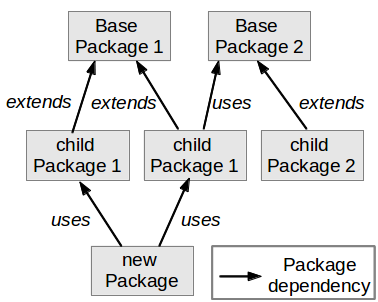
\includegraphics[scale=1]{images/package_hierarchy.png}
\caption{An example hierarchy of packages}
\label{fig-pack-hier}
\end{figure}

From a functional point of view a dependency can generally represent one of these two alternatives relationship:
\begin{itemize}
\item an "extension" relation : a child package \textbf{extends} a base package if it provides some functionalities that specialize/extends those of the base package. This is a typical relationship when a library extends the class hierarchy provided by a library of the parent package, or/and when a more specialized/complete version of an application/component is provided.
\item a "use" relation : a child package \textbf{uses} a base package if it provides new functionalities built onto those provided by the base package. This is the case when new libraries are using more basic ones or when new applications/component are built using existing applications/components.
\end{itemize}


\paragraph{Packages Dependencies guideline:}
\begin{itemize}
\item If a package has some dependencies induced by lower levels of the class hierarchy, prefer making a package for the higher level with less dependencies, and one or more dependent "extension" packages for the lower levels, each of them with the strict minimum required dependencies.
\item Prefer an atomic structuring of package by limiting the number of software artefacts generated by a package. Typical use is one package per application or per library (this advice does not targets test cases and examples).
\item When developing a component for a given middleware (ROS, OROCOS, etc.) always put the functional code (library) in one package and extend this package each time a component is built from this code.
\item Cyclic dependencies are forbidden.
\item Dependencies to multiple packages are allowed but the developer should keep in mind to have the lowest possible number of dependencies for a given package.
\item Making several packages dependent from a same package is encouraged when these dependencies put in place an "extension" relationship.
\item Limit the number of hierarchical level to the strict necessary. As a global guideline we discourage having more than 4 hierarchical levels for the "extension" relationship to keep the extension hierarchy understandable. 
\end{itemize}



\section*{Conclusion}

Concerning package development, developers have to refer to dedicated document explaining coding rules and general code development guidelines.

\section*{POUBELLE}

\textbf{framework} :  a framework is a site where are deployed packages versions, consisting in a set of header files, libraries, executables, script-like files, tutorials, etc., without development artifacts (source code, build files, etc.). A framework embeds one or more stable versions of a given package that have been previously released by the package developers, allowing the user to choose which version he wants to use (for instance to compile a package in development).
 The workspace also provides categories : each category defines a specific subject that helps classifying packages/frameworks. For instance the category sensor will reference all packages or frameworks that implement the driver of a sensor. Categories can be hierarchically refined into sub categories for instance the category camera refines the category sensors. Categories can be viewed as lists of links that target frameworks/packages. The process of classification of packages is itself coming from package description (i.e. a package specifies the categories it belongs to).
 
 
GIT TAGS
 
\paragraph{Handling tags for version numbers:}
\begin{itemize}
\item creating the version number (annotated tags):
\linebreak \texttt{git tag -a v1.2.3 -m"<small description of the version>"}
\item listing all available versions: 
\linebreak \texttt{git tag -l 'v*'}
\item showing the information of a given version: 
\linebreak \texttt{git show v<version number>}
\item getting the released version in package history: 
\linebreak \texttt{git checkout tags/v<version number>}
\end{itemize}


It is also possible to apply tags to certain moment of the package's life in order to register important dates of package state and retrieve this state at any moment in the future. We define two other tag patterns to do so : publication tags, representing software developed to do experiments in the frame of a scientific publication and demo tags used to target versions that match working technical demonstrations. Demo and publication tags relies on last released version number and had specific information:
\begin{itemize}
\item \textbf{publication tags pattern} have the shape: \linebreak \texttt{pX.Y[.Z]-<journal-or-conference>-<year>}.
\item \textbf{demo tags pattern} have the shape:
\linebreak \texttt{dX.Y[.Z]-<name of demo>-<year>}.
\end{itemize}
 
GIT BRANCHING
 
\paragraph{Handling feature branches in GIT:}
\begin{itemize}
\item Creating a feature branch:
\linebreak \texttt{git checkout -b <feature name> develop}
\item Listing available branches:
\linebreak \texttt{git branch -a}
\item Incorporating a finished feature on develop:
\linebreak \texttt{git checkout develop}
\linebreak \texttt{git merge --no-ff feature-<feature name>}
\linebreak \texttt{git branch -d  feature-<feature name>}
\linebreak \texttt{git push origin develop}
\end{itemize}


\pagebreak
\paragraph{Handling hotfixes branches in GIT:}
\begin{itemize}
\item Creating a hotfix branch:
\linebreak \texttt{git checkout -b hotfix-<patch version> master}
\item Incorporating a finished hotfix on master and develop:
\linebreak \texttt{git checkout master}
\linebreak \texttt{git merge --no-ff hotfix-<patch version>}
\linebreak \texttt{git tag -a <patch version>}
\linebreak \texttt{git push origin master}
\linebreak \texttt{git checkout develop}
\linebreak \texttt{git merge --no-ff hotfix-<patch version>}
\linebreak \texttt{git branch -d  hotfix-<patch version>}
\linebreak \texttt{git push origin develop}
\end{itemize}


COLLABORATIVE WORKING

When an administrator decides to affect a pool of developers to the development of a package:
\begin{enumerate}
\item he first \texttt{clones} the official repository of the package into a private access area on the server, that is accessible (via ssh access) only to this pool of developers. 
\linebreak \texttt{ssh <private area>}
\linebreak \texttt{git clone <address of the package official repository>}
\item Second, he creates one or more feature branches as described in previous section.
\linebreak \texttt{git checkout -b <feature name> develop}
\item Third, all developers in turn \texttt{clone} this private repository into their own work station so that they can work locally and update (\texttt{push/pull})the server version of the private repository.
\linebreak \texttt{git clone <address of the package private repository>}
\item When features development is done or aborted, the administrator deletes 
the private repository on server by simply deleting the repository's folder and removing access to the users if necessary.
\linebreak \texttt{ssh <private area>}
\linebreak \texttt{rm <package private repository folder>}
\end{enumerate}
 
\begin{itemize}
\item Creating a local version of a package repository:
\linebreak \texttt{cd <path to workspace>/packages/}
\linebreak \texttt{git clone <address of the package official repository>}
\item Registering a private repository for a given package on administrator workstation:
\linebreak \texttt{cd <path to workspace>/packages/<package>}
\linebreak \texttt{git remote add <private repository name> <private repository address>}
\item To get the state of a private repository, without merging the result with administrator's local branches:
\linebreak \texttt{git fetch <private repository name>}
\item To remove a reference to a private repository (just after/before deletion of the repository by hand):
\linebreak \texttt{git remote rm <private repository name>}
\end{itemize} 

PACKAGE DESCRIPTION

The package is described in the \textbf{package.manifest} file. This file centralizes all meta-information about the package, notably considering authoring and licensing aspects. This file looks like this for a given package named "mypack":
\begin{verbatim}
<package name="mypack" address="git@idh.lirmm.fr:mypack.git"
license="LGPL" version="1.2.5">
<description>
	//short package description
</description>
<category name = "sensor/camera" />
<category name = "image/processing" />
<author name="Robin" role="administrator" institution="LIRMM" />
<author name="Sebastien" role="developer" institution="LIRMM" />    
<author name="Francois" role="developer"institution="LIRMM" />
<dependency name="myotherpack" min_version="0.4"
address="git@explore.lirmm.fr:otherpack.git"/>
<installer platform="ubuntu" version="1.0.2"
address="ftp://ftp.gforge.fr/mypack-1.0.2-ubuntu.tgz" />
<installer platform="ubuntu" version="1.2.0" 
address="ftp://ftp.gforge.fr/mypack-1.2.0-ubuntu.tgz" />
<installer platform="macosx" version="1.2.0" 
address="ftp://ftp.gforge.fr/mypack-1.2.0-macosx.tgz" />
</package>
\end{verbatim}

\paragraph{Data Type Definition:}
\begin{verbatim}
<!DOCTYPE package [

<!ELEMENT package (description, category*, author+, dependency*, 
installer*)>
<!ELEMENT description (CDATA)>
<!ELEMENT category (EMPTY)>
<!ELEMENT version (EMPTY)>
<!ELEMENT license (EMPTY)>
<!ELEMENT author (EMPTY)>
<!ELEMENT dependency (EMPTY)>
<!ELEMENT installer (EMPTY)>

<!ATTLIST package name CDATA #REQUIRED>
<!ATTLIST package address CDATA #REQUIRED>
<!ATTLIST category name CDATA #REQUIRED>
<!ATTLIST version release CDATA #REQUIRED>
<!ATTLIST license type CDATA #REQUIRED>
<!ATTLIST author name CDATA #REQUIRED>
<!ATTLIST author role CDATA #REQUIRED>
<!ATTLIST author institution CDATA #IMPLIED>
<!ATTLIST dependency name CDATA #REQUIRED>
<!ATTLIST dependency min_version CDATA #IMPLIED>
<!ATTLIST dependency max_version CDATA #IMPLIED>
<!ATTLIST dependency address CDATA #REQUIRED>
<!ATTLIST installer platform CDATA #REQUIRED>
<!ATTLIST installer version CDATA #REQUIRED>
<!ATTLIST installer address CDATA #REQUIRED>
]>
\end{verbatim}


\paragraph{Explanations:}
\begin{itemize}
\item The \texttt{<package>} markup is the root of the XML description. The \texttt{name} parameter is the same as the package folder name and \texttt{address} specifies where to find the official git repository containing package sources. \texttt{version} defines the last released version of the package (the last version available on master branch with tag containing the given version number). Only release version are referenced, not demo or publication versions. The \texttt{licence} attribute specifies which license applies to the package's content.
\item the \texttt{description} markup contains a brief description of the package content.
\item The \texttt{<category>} markups defines in which categories the package is classified (i.e. topics addressed by the package).
\item The \texttt{<author>} markups list all developers that participate to the development of the package since its creation. Developers have one of the following roles :
\begin{itemize}
\item \textbf{developers} are basic users of the package, they can modify any development artefacts (source code, interface, launch, tests, cmake files, etc.) on feature branches.
\item \textbf{administrators} have the right to do quite anything on the package, they have same rights as developers but also have other particular rights : merging features branches into develop branch ; declaring new production version release (merge on master branch, either from develop or hotfix branches) ; declaring new available installers ; declaring new categories for the package ; changing license or server where the official repository can be found.
\end{itemize}
\item the \texttt{dependency} markups declare names and address of packages that are used by the current package. Dependencies are useful information for the developer to find and install packages that provide code (e.g. a library, an executable) used by the current package. Min and max version of the required package can be specified, which is an useful information when deploying a binary version of the package.
\item the \texttt{installer} markups declare OS installers for binaries of the package. Each installer matches a given version of the package, a given platform and an address where to find the installer. Instead of using a git version of the package, another package that depends on it can simply be bound to an adequate binary version.
\end{itemize}

\paragraph{Remarks about usage of this file:}

This file centralizes information for developers of the package. It must to be update each time it is necessary:
\begin{itemize}
\item When a new production version is released and the master branch is tagged, the \textit{released} number (in \texttt{version} markup) must be incremented accordingly by an administrator.
\item Each time a new developer contribute to the package it can be automatically added to the list of authors.
\item The license specified must conforms to the available licenses (see workspace).
\item Whenever an administrator wants to make available an OS installer for the package's binaries, he simply adds it to the package.manifest file.
\end{itemize}  
 
 
The development process of a package is always initiated by administrators:
\begin{itemize}
\item because they know which packages are already available and so which one can be used or extended in the frame of a master/PHD student or postdoc job.
\item because they know who is already working on similar or complementary software.
\item because they know which kind of constraints apply to code produced in the laboratory (licenses, access restriction, etc.)
\end{itemize} 
They are so the only persons that can truly:
\begin{itemize}
\item orient and help developers to increase their productivity by reusing existing code.
\item optimize collaboration between developers.
\item centralize the whole process.
\end{itemize} 


Nearly all the development process takes place in developers/administrators workstations, around the private repository:
\begin{itemize}
\item Implementing package features.
\item Updating the current \textbf{feature branch} on private repository with modifications made on the \textbf{develop} branch. Features never update between each other but only around \textbf{develop} branch. 
\item Managing features branches integration when feature development is finished (see previous section).
\item Creating Hotfix branches and implementing hotfixes in them (see previous section).
\end{itemize}


\paragraph*{Frameworks} 
Frameworks are simple folders that contain binary version of package, in other word the installation of packages' binaries has to be done in frameworks. A framework is a "screen-shot" of a given package at a given time of its lifetime : it contains the functionalities (executables, scripts, libraries, etc.) provided by the package's version, but no development artefact (no source or build file for instance).

The notion of framework (partly coming from mac osx frameworks) as many advantages as regards to classical system installation process :
\begin{itemize}
\item Frameworks help grouping related resources together. This grouping makes it easier to install, uninstall, and locate those resources. For instance libraries and their related headers are logically group in the same place as opposed to system install.
\item Frameworks can include a wider variety of resource types than just libraries or headers. For example, a framework can include any relevant documentation, html-based API or configuration files.
\item Multiple versions of a package can be included in the same framework, allowing a smart management of backward compatibility.
\end{itemize}

the \textbf{categories} folder is structured according a set of topics, each topic being itself a folder that in turn contains either other subcategories or \textbf{links to frameworks}. \textbf{categories} only goal is to help finding available packages (under binary form) according to a given theme. Considering a category, packages that are relevant for the theme it defines are referenced as links (symbolic relative links in Linux) to frameworks folders.


\paragraph{Rules for the modification of the repository:}
\begin{itemize}
\item .gitignore cannot be modified.
\item No new direct subfolder or file of the workspace root can be created or removed.
\item files (package references, licenses definitions) can be added or removed only by administrators.
\end{itemize}



\subsubsection{Deployment in frameworks}

Frameworks are simple repositories in which the binary code or more generally the code usable by third parties is installed. The install process of a package  version in its framework is made either :
\begin{itemize}
\item by package developers using \texttt{make install}, after the compilation phase. The package version is then the current version
\item by package users, after downloading the archive of the package, using OS specific primitives (e.g. \texttt{dpkg -i}).
\end{itemize}
In both cases, the \textbf{CMakeList.txt} file of a given package defines the way this package is deployed (according to rules defined in this document), either:
\begin{itemize}
\item directly, by generating the \texttt{make install} procedure.
\item indirectly, using \textit{cpack} toolset, by generating the \textbf{OS installer} that does the same job, but without having to get access to the package repository.
\end{itemize}


\subsubsection{General policy to manage many package versions}

The following rules should be applied whenever developers want to install a given package version:
\begin{itemize}
\item Given a package version with given major and minor version numbers, its more recent patch version should always be used. If a new patch version becomes available (e.g. 1.4.2 after a hotfix on 1.4.1) it should replace older patch versions (e.g. 1.4.0 or 1.4.1) if any installed in the package framework. This ensures the developer to use a version with less bug or security problems.
\item When a new backward compatible version (e.g. 1.5.0) of a package is to be installed, it may replace the previous version (e.g. 1.4.2) or be simply added to the framework. Most of time it is preferable to test effective compatibility between this new version and the code that was using the old version.
\item When a new non backward compatible version of a package is to be installed (e.g. 2.0.0 while 1.4.2 is already installed), it should not immediately replace older versions. The package version is simply added to the package framework, which ensures that other packages can still work with an older version already installed.
\end{itemize}

\paragraph*{When to install ?}
Generally, there are two main case when developer want to install a package version:
\begin{itemize}
\item they want to install software artefacts (libraries, scripts, etc.) coming from a package they are currently developing, in order to use them. In this case, package version is installed in the \textbf{own} folder of the framework. This folder is updated each time they compile their package.
\item  they develop or use a package that requires other packages with version constraints. For a given required package, a released version with number contained between its min and max version constraints has to be installed. In the allowed "interval of versions", the last backward compatible version with last patch version should be installed.
\end{itemize}

\paragraph*{How to install ?}
There are basically two way to install a given package version:
\begin{itemize}
\item from package repository: the developer has to go back to the given version in history (on master branch) and install it.
\linebreak \texttt{git checkout master}
\linebreak \texttt{git checkout tags/v<version number>}
\linebreak \texttt{cd build}
\linebreak \verb|{cmake .. - DCMAKE_INSTALL_PREFIX=../../frameworks/|
\linebreak \verb|<package name>/<version number>/|
\linebreak \texttt{make}
\linebreak \texttt{make install}
\item from an OS installer: it depends on the installer used but the install prefix has to be specified quite the same way as previously.
\end{itemize}

\subsection{Referencing Packages in Workspace}

To reference available packages potentially accessible in the workspace, we use the \textbf{references} folder in which administrators put \textbf{package.manifest} files. In the workspace these files are used to tell to users which packages are available and where they can be found. When a package administrator wants to make the package available to others, he must add the corresponding \textbf{package.manifest} in the \textbf{references} folder of its workspace and commit the changes to the workspace. All users will then know the package existence whenever they update their workspace. When a package definitively become obsolete, the corresponding manifest file is removed from the \textbf{references} folder and the changes into the workspace are committed.

\paragraph{Basic commands}
\begin{itemize}
\item Referencing a package :
\linebreak copying the package.manifest file into the references folder of the workspace, and \textbf{rename it} in <name of package>.manifest (name of packages are supposed to be unique).
\linebreak \texttt{git add <package name>.manifest}
\linebreak \texttt{git commit -m "<package manifest file> is now referenced"}
\linebreak \texttt{git push origin master}
\item Updating available references (when updating the workspace):
\linebreak \texttt{git pull origin master}
\item Dereferencing a package
\linebreak \texttt{git rm <package name>.manifest}
\linebreak \texttt{git commit -m "<package manifest file> is no more referenced"}
\linebreak git push origin master
\end{itemize}

\subsection{Licensing packages}

The licensing of packages has to be done according to a general politics of the laboratory, team or sub-group. License is let free to their decision and constraints, nevertheless, as software licenses are the same for everybody, licenses definitions are shared between all people.

The \textbf{licenses} folder contains definitions for all licenses that are available for use in package description. Each license is defined in a specific file that looks like this for the GPLv3 license (file name is "GNUGPLv3.license") :
\begin{verbatim}
<license id="GPLv3" fullname="GNU General Public 
License version 3" organization="Free Software Foundation"/>
<description>
/*
* <package_name> : <package_short_description>
* Copyright (C) <year>  <authors_name>

* This program is free software: you can redistribute it and/or modify
* it under the terms of the GNU General Public License as published by
* the Free Software Foundation, either version 3 of the License, or
* (at your option) any later version.
*
* This program is distributed in the hope that it will be useful,
* but WITHOUT ANY WARRANTY; without even the implied warranty of
* MERCHANTABILITY or FITNESS FOR A PARTICULAR PURPOSE.  See the
* GNU General Public License for more details.

* You should have received a copy of the GNU General Public License
* along with this program.  If not, see <http://www.gnu.org/licenses/>.
*/
</description>
<legalterms>
//input the full legal terms of the license here
</legalterms>
</license>
\end{verbatim}


\paragraph{Data Type Definition:}
\begin{verbatim}
<!DOCTYPE license [

<!ELEMENT license (description, legalterms)>
<!ELEMENT description (CDATA)>
<!ELEMENT legalterms (CDATA)>

<!ATTLIST license id CDATA #REQUIRED>
<!ATTLIST license fullname CDATA #REQUIRED>
<!ATTLIST license organization CDATA #REQUIRED>
]>
\end{verbatim}


\paragraph{Explanations:}
\begin{itemize}
\item the \texttt{<license>} markup is the root of the XML description : it gives the short name of the license used as an identifier (\texttt{id}) in the package description as well as its complete legal name (\texttt{fullname})and the name of the \texttt{organization} that wrote it.
\item the \texttt{<description>} markup contains a short text that has to be put by developers into any file used in the package (source, interface, test, etc.). Some part have tags with "<" and ">" characters : this is where package specific informations (name, authors, short description etc.) is written by developers.
\item the \texttt{<legalterms>} markup contains the full legal text of the license. Thanks to this text a license text file can be generated and added with redistribution of packages (e.g. both in repositories and installers).
\end{itemize}

\paragraph{Important remarks:} 
\begin{itemize}
\item As a package has one license only, using different licenses requires to define different package.
\item If a package has one license at a time this license can evolve along time.
\item Only administrators can add/remove/modify license files in the workspace.
\end{itemize}


\subsection{Categorizing packages}

When developing it is often useful to know which package provide some useful things relative to one or more topics. The aim of the \textbf{categories} folder is to standardize the classification and the finding of packages relevant for given concerns.

The \textbf{categories} folder is structured into subfolders that describe known categories. Each category folder is itself structured the following way:
\begin{itemize}
\item sub folder describes sub categories. A sub category refines the topic of its containing category. For instance folders \textbf{arms} and \textbf{wheeled vehicles} are contained in the category folder \textbf{robot}. These sub categories can in turn be refined the same way.
\item symbolic links represent target packages of the category. The name of the link is simply the name of the package, the target of the link is a given package framework. The target itself is always expressed as a \textbf{relative path} from the containing category folder to the target framework. By default these links target nothing in the file system as long as the package's framework has not been installed in the \textbf{frameworks} folder.
\end{itemize}

\paragraph*{Remark:} 
a same package can be targeted by more than one link: it means that the package belongs to different (sub)categories according to the different point of view of the developers. Doing so, anyone can have his own point of view of the package depending on its center of interest.
\linebreak

To organize the development, defining some "standard categories" should help developers to classify their packages. This requires to list categories of code that is useful for robotic applications development. For instance :
\begin{itemize}
\item sensors
\begin{itemize}
\item vision
\begin{itemize}
\item cameras
\item kinects
\item lasers
\end{itemize}
\item force sensors
\item encoders
\end{itemize}
\item robots
\begin{itemize}
\item arms
\item wheeled vehicles
\item humanoids
\end{itemize}
\item simulators
\item navigation
\begin{itemize}
\item cartography
\item positioning
\end{itemize}
\item planning
\begin{itemize}
\item mission
\item path
\item trajectory
\end{itemize}
\item middleware
\begin{itemize}
\item ros
\item contract
\item orocos
\end{itemize}
\end{itemize}

Of course categories can evolve/change along time, when developers want new categories.

\subsubsection{Working with categories}

The only people that can modify \textbf{categories} folder are package administrators. Each time a new package is created, developers define which are its relevant categories and wrote them in the package.manifest file of the package. When an administrator of a package wants to reference it :
\begin{itemize}
\item he first copy/rename the package.manifest file into the \textbf{references} folder.
\item according to the relevant categories of tha package defined in the manifest, he:
\begin{itemize}
\item creates new (sub)category folders in the the \textbf{categories} folder of its workspace, if the corresponding categories do not exist.
\item creates as many symbolic links that target the package framework as there are relevant categories for the package and put these links into the adequate category folders.
\end{itemize}
\item once done he commits its workspace.
\end{itemize}

From developers point of view, categories just help finding packages that are relevant for given topics. Each time they update their workspace, all available categories and classification of packages according to categories are updated. 

To search packages, they can simply navigate in the file system of the \textbf{categories} folder. 
\begin{itemize}
\item if the package is already installed in the \textbf{frameworks} folder he can simply follow the link.
\item otherwise the link is broken, and the developer has to install the corresponding package.
\end{itemize}

\end{document}